% !TEX root = ../YourName-Dissertation.tex
\Appendix{Figures}

\section{Chapter 1}
\begin{figure}[H]
    \centering
    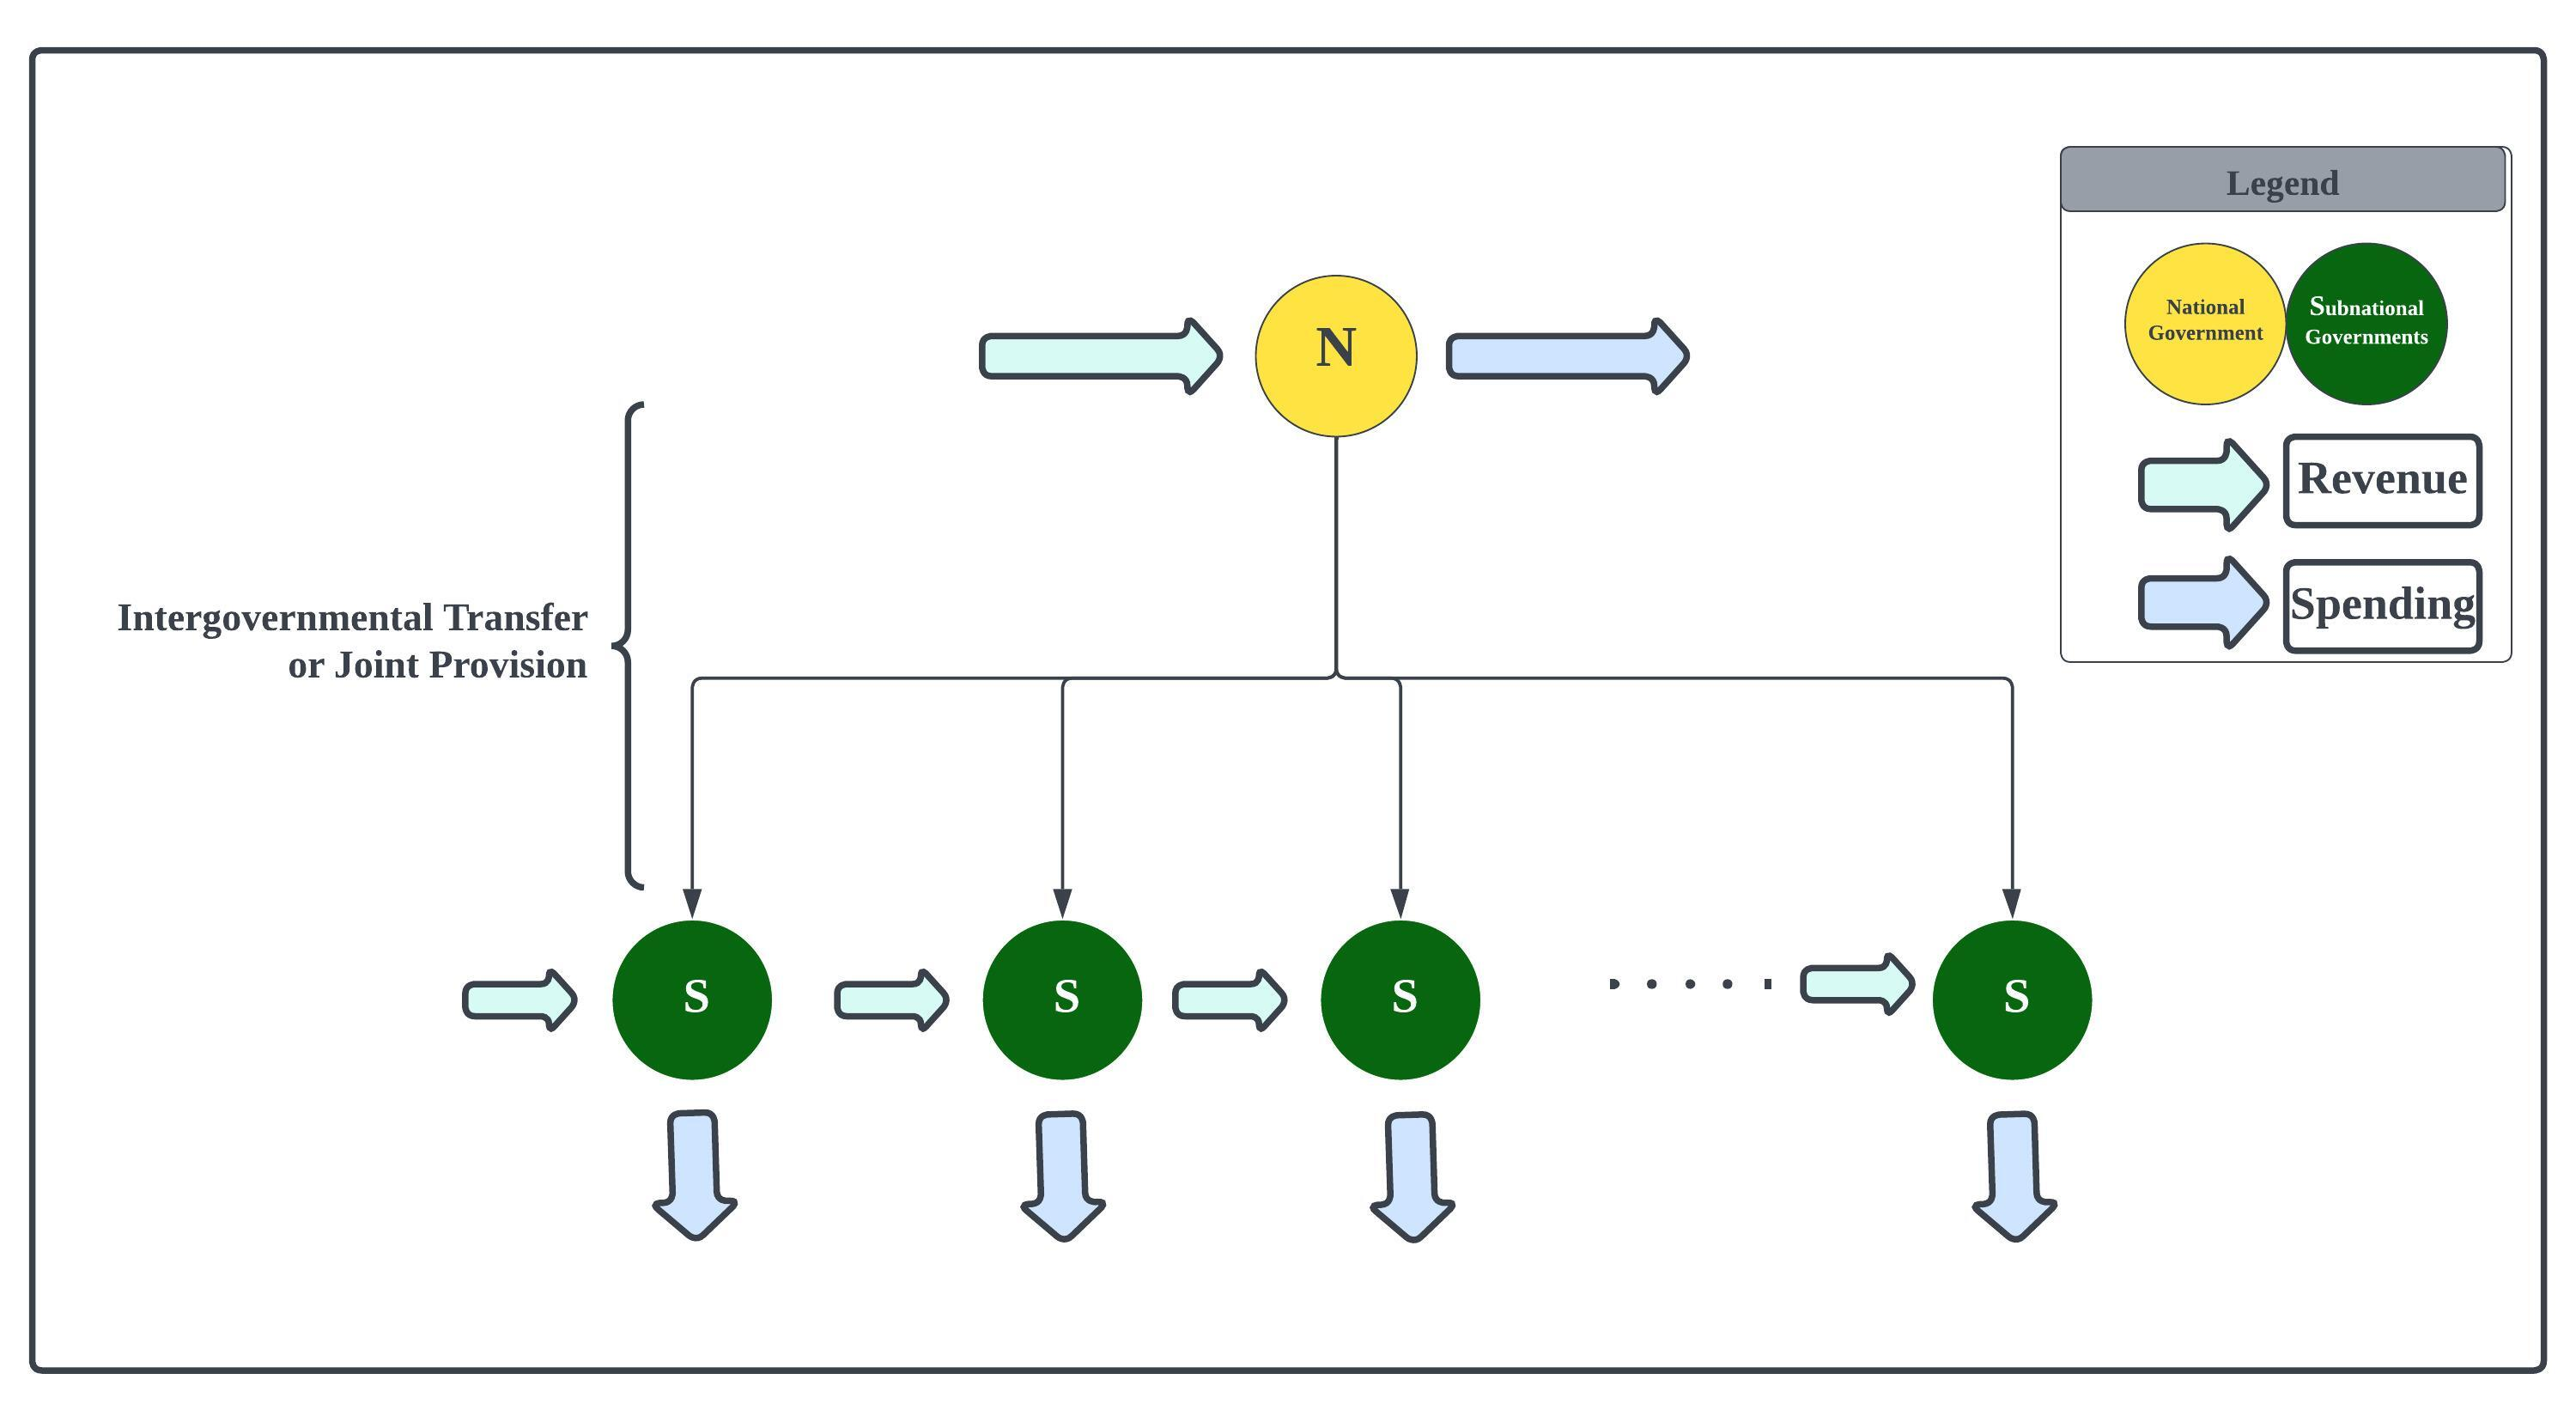
\includegraphics[scale=0.6]{Chapter-1/Figures/fiscal federalism.jpeg}
    \caption[Fiscal Federalism Structure]{Fiscal Federalism Structure
        \texttt{} }
    \label{Figure 1.1}
\end{figure}

\clearpage

\begin{figure}[H]
    \centering  %居中
    \subfigure[Federal Expenditure]{   %first subfigure
        \begin{minipage}{7cm}
            \centering    %子图居中
            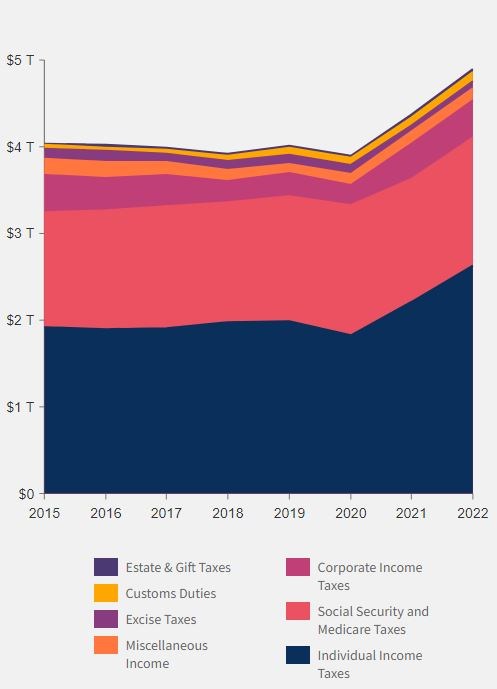
\includegraphics[scale=0.52]{Chapter-1/Figures/source of federal revenue.JPG}  %以pic.jpg的0.5倍大小输出
        \end{minipage}
    }
    \subfigure[State and Local Expenditure]{ %second subfigure
        \begin{minipage}{7cm}
            \centering    %子图居中
            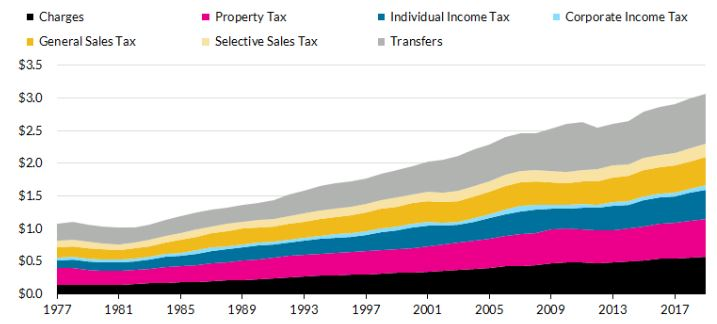
\includegraphics[scale=0.52]{Chapter-1/Figures/source of state and local revenue.JPG}%以pic.jpg的0.5倍大小输出
        \end{minipage}
    }

    \caption[Fluctuation of Revenue Structure]{Fluctuation of Revenue Structure of three level governments.Data Source: US Urban Institute Dataset  }    %caption for whole figure
    \label{Figure A.1}
\end{figure}

\clearpage

\begin{figure}[H]
    \centering
    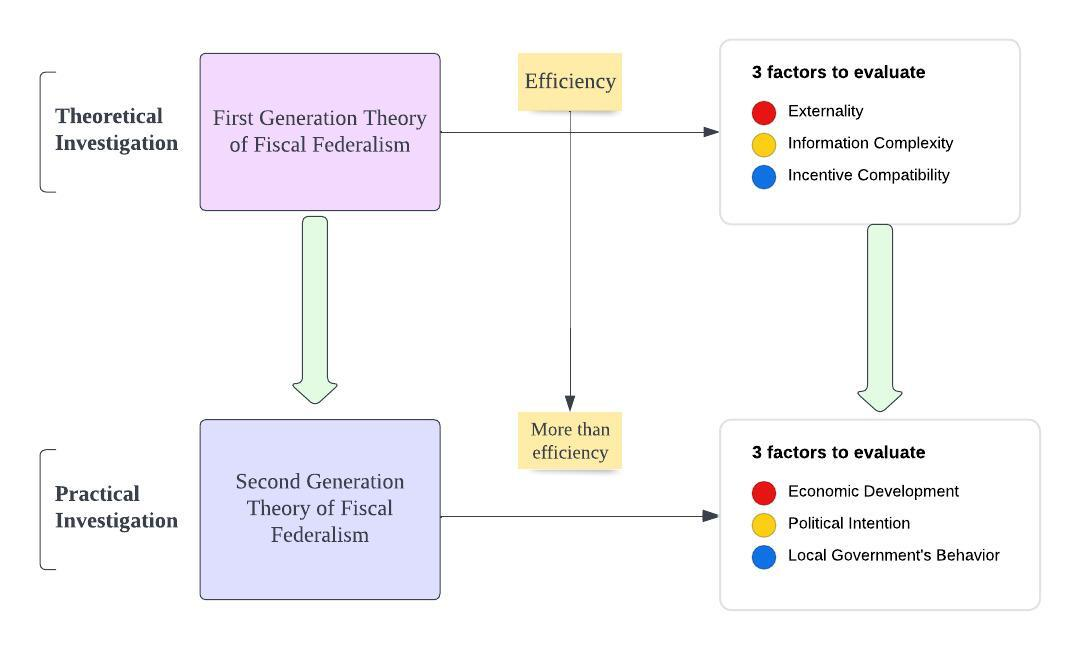
\includegraphics[scale=1]{Chapter-2/Figures/how to evaluate the fiscal federalism.jpeg}
    \caption[How to evaluate the fiscal federalism]{How to evaluate the fiscal federalism
        \texttt{} }
    \label{Figure 1.2}
\end{figure}

\clearpage

\begin{figure}[htbp]
    \centering
    \subfigure[Source of Federal Revenue]{
        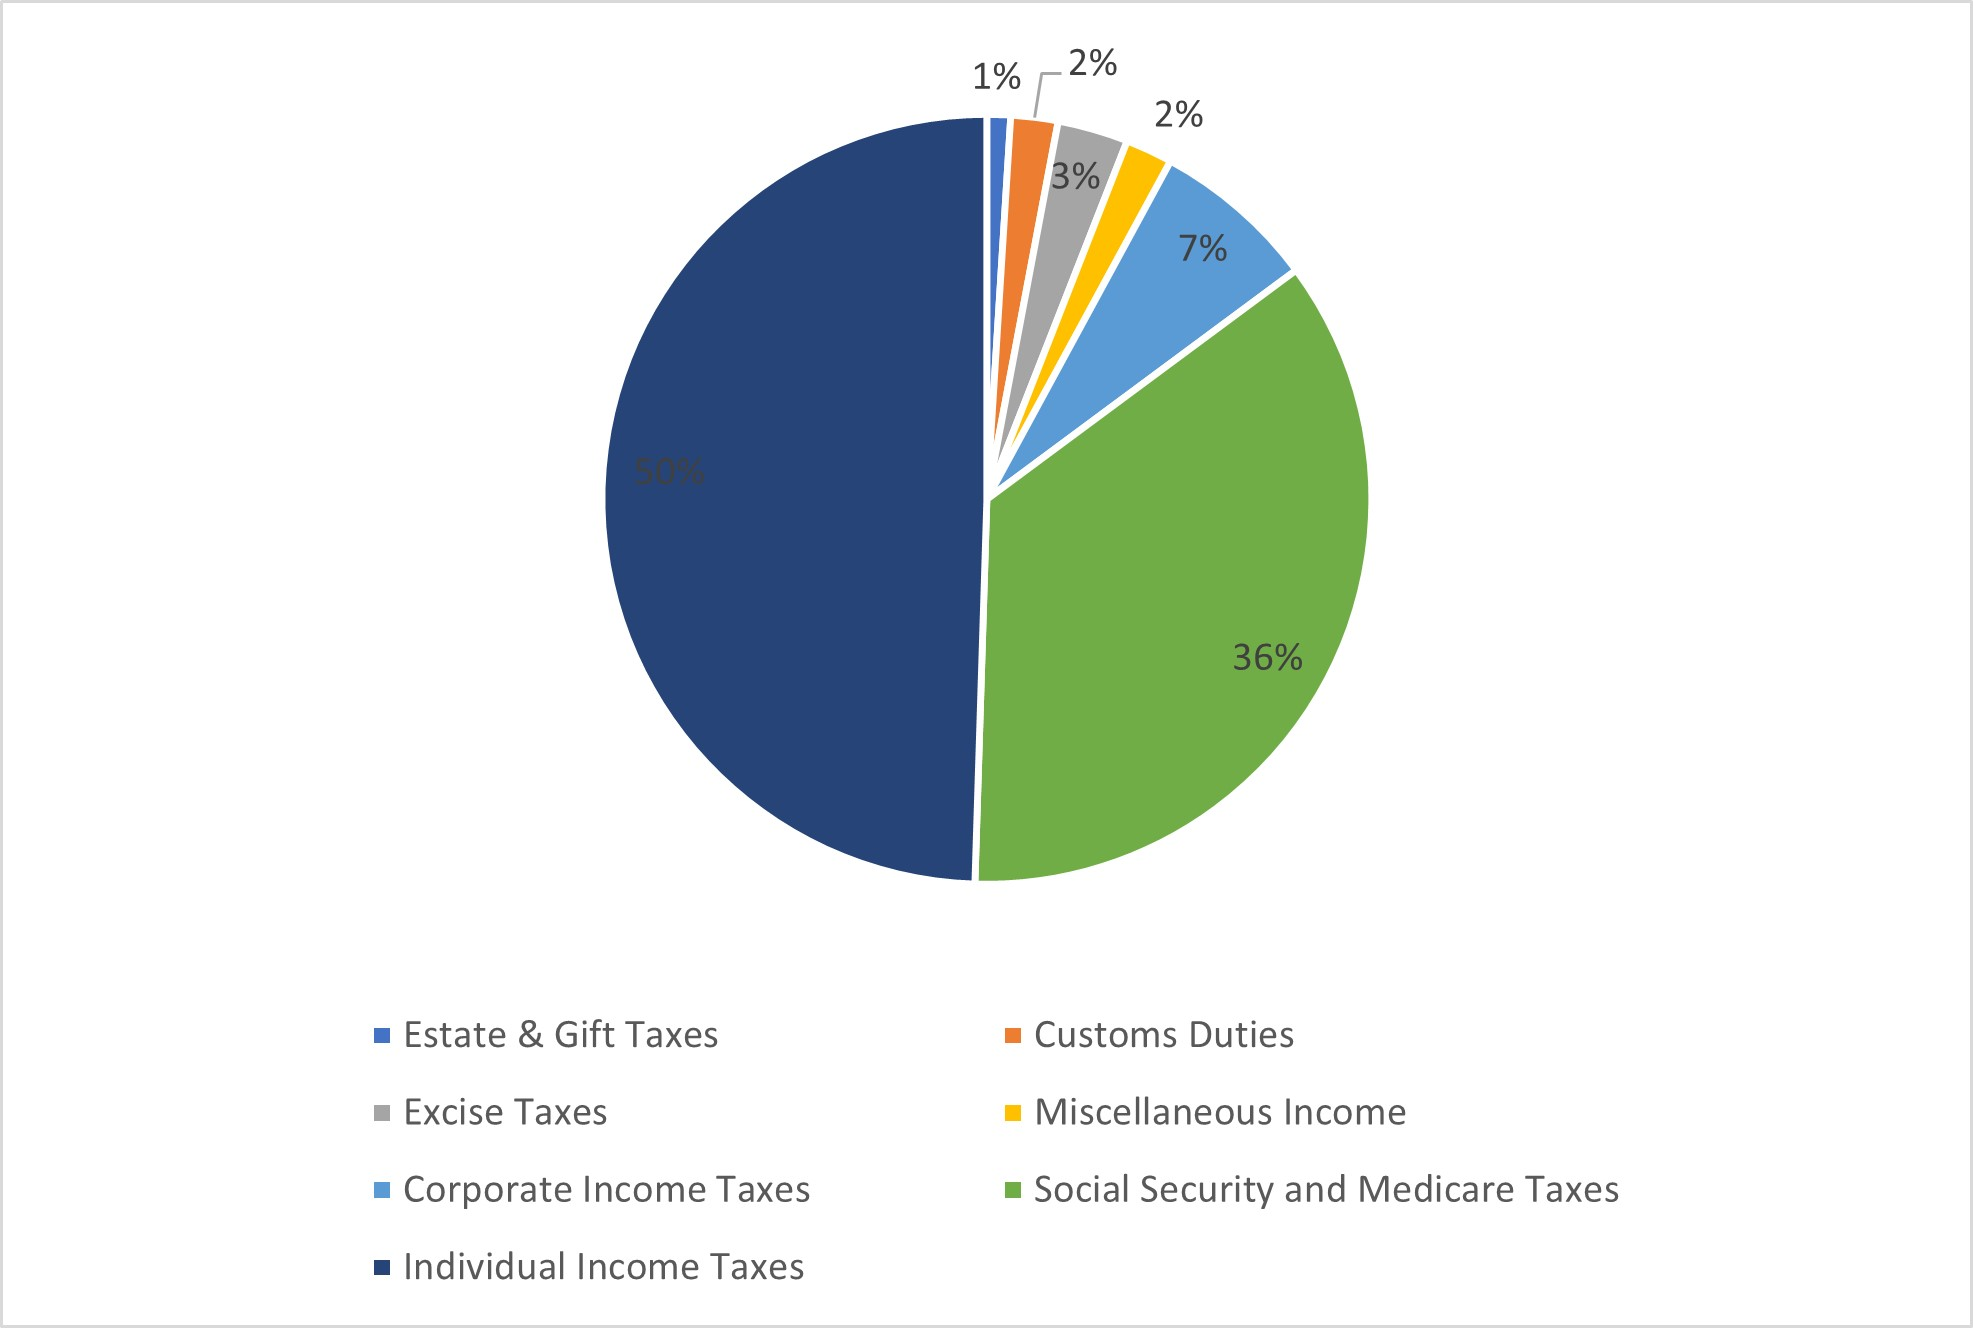
\includegraphics[width=0.31\textwidth]{Chapter-1/Figures/source of federal general revenue.jpg}}
    \subfigure[Source of State Revenue]{
        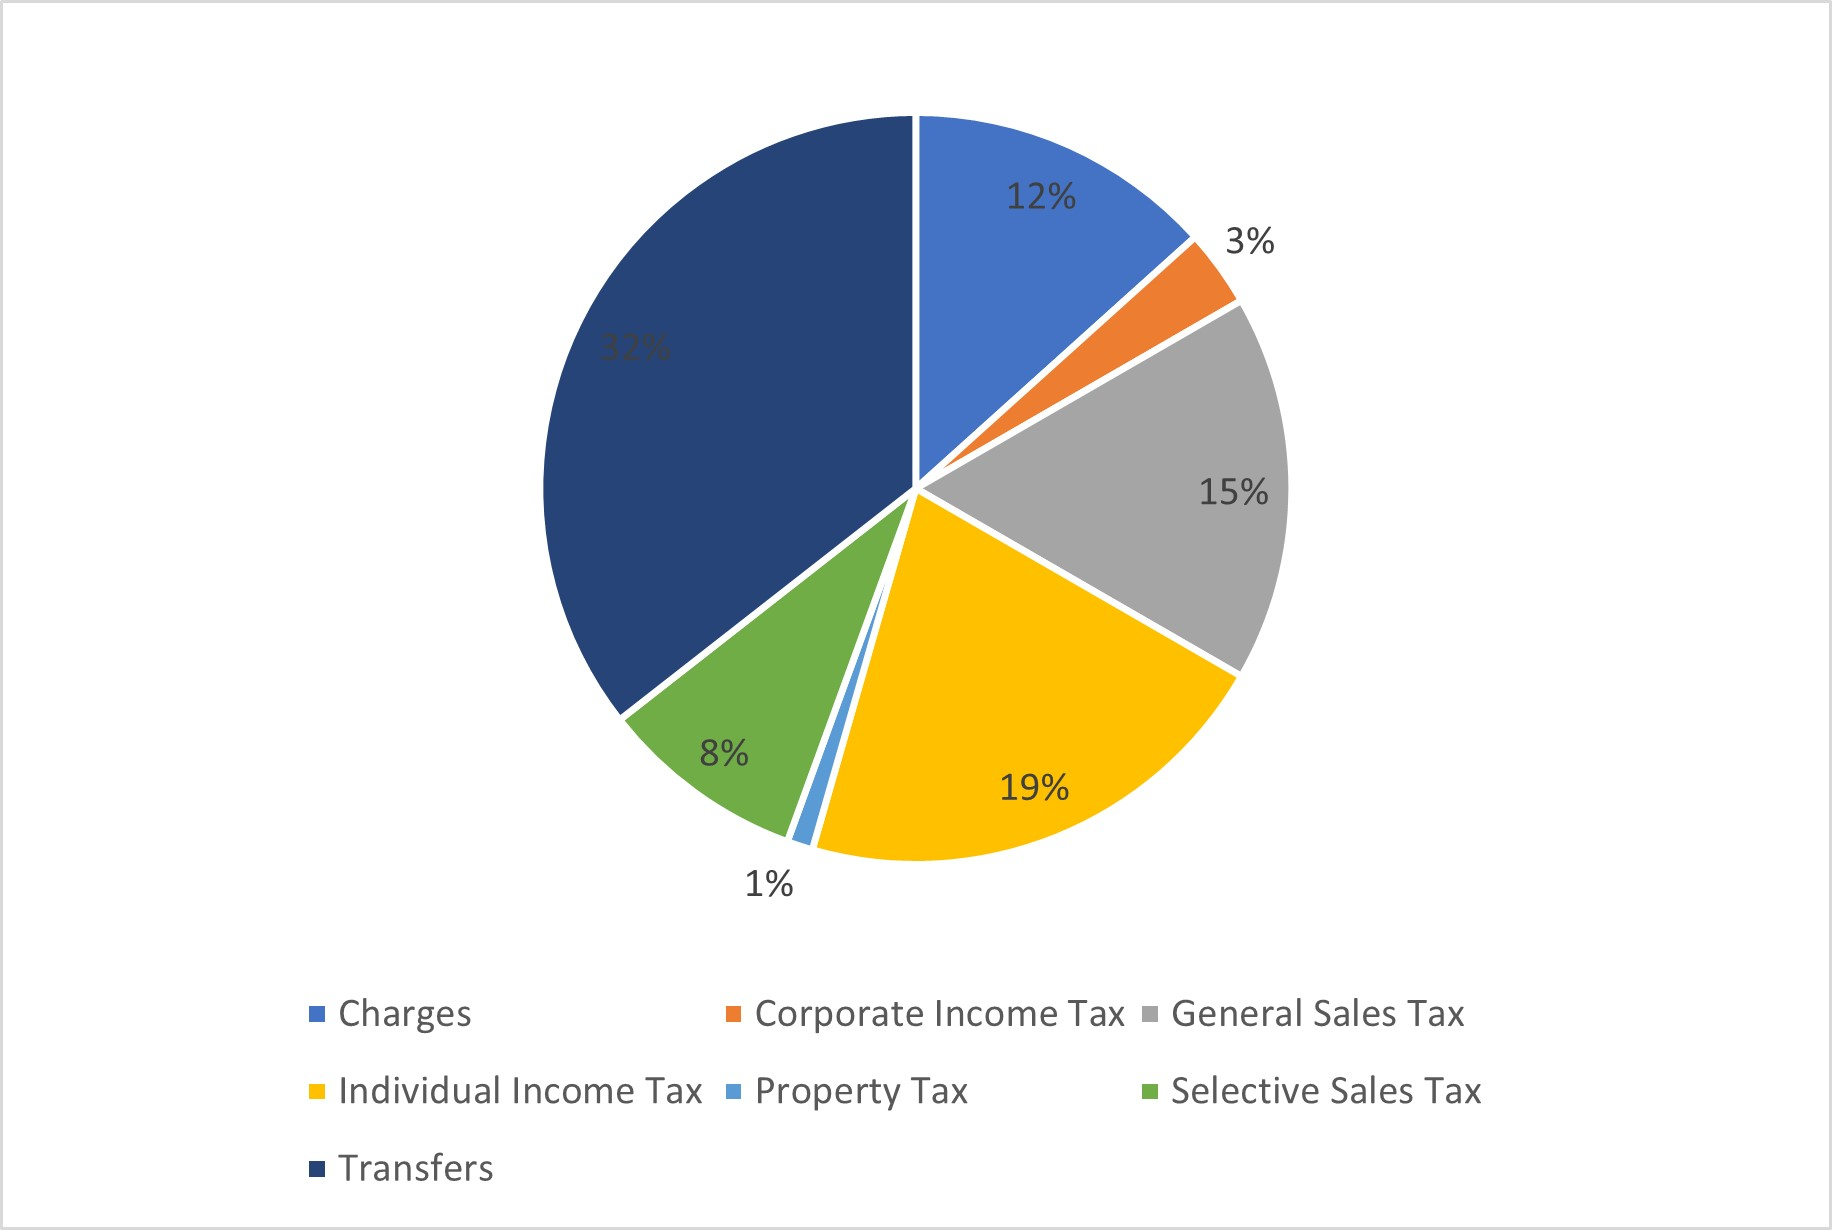
\includegraphics[width=0.31\textwidth]{Chapter-1/Figures/source of state general revenue.jpg}}
    \subfigure[Source of Local Revenue]{
        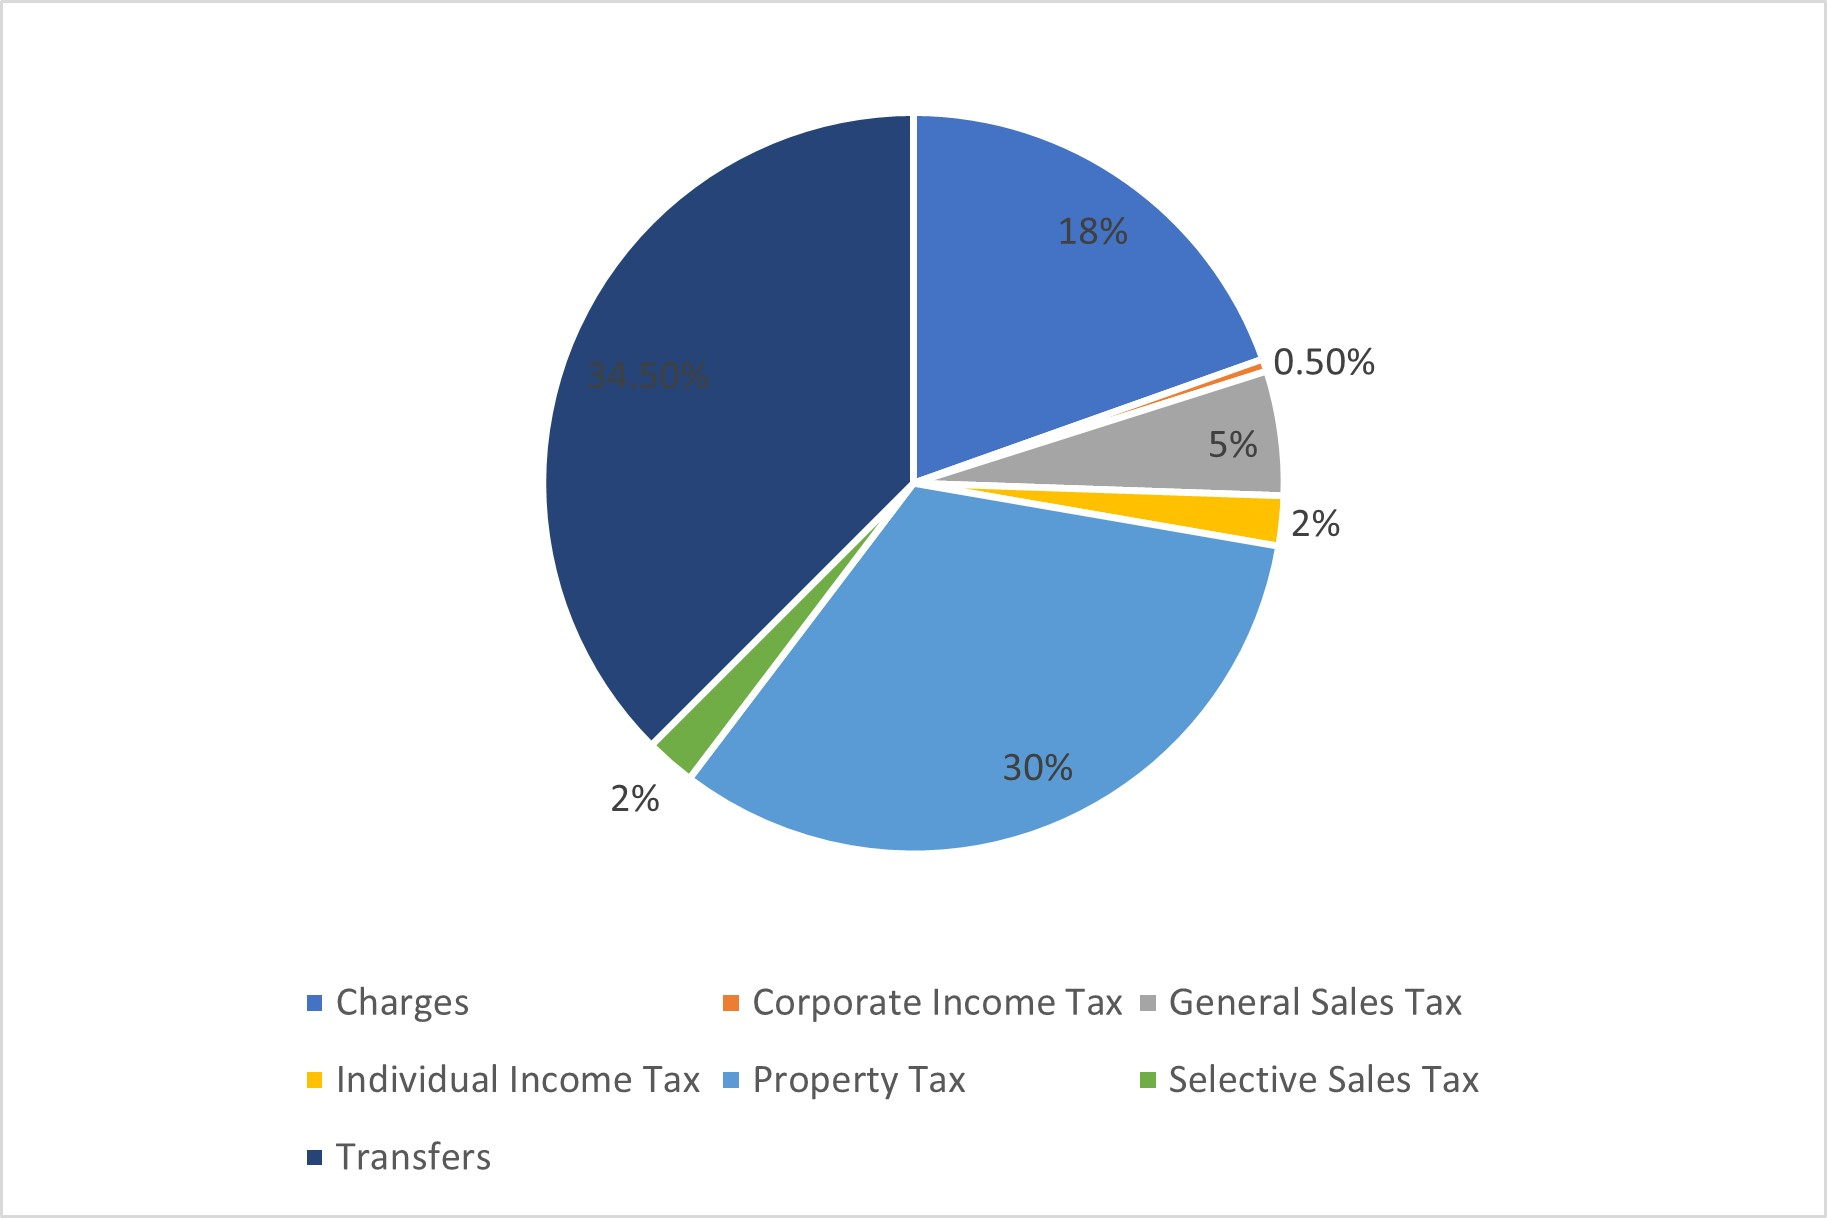
\includegraphics[width=0.31\textwidth]{Chapter-1/Figures/sources of local general revenue.jpg}}
    \caption[Source of Revenue for Multiple Level of Governments in 2019]
    {Source of Revenue for Multiple Level of Governments}
    \label{sourceofreveune}
\end{figure}

\begin{figure}[H]
    \centering  %居中
    \subfigure[Federal Expenditure]{   %first subfigure
        \begin{minipage}{7cm}
            \centering    %子图居中
            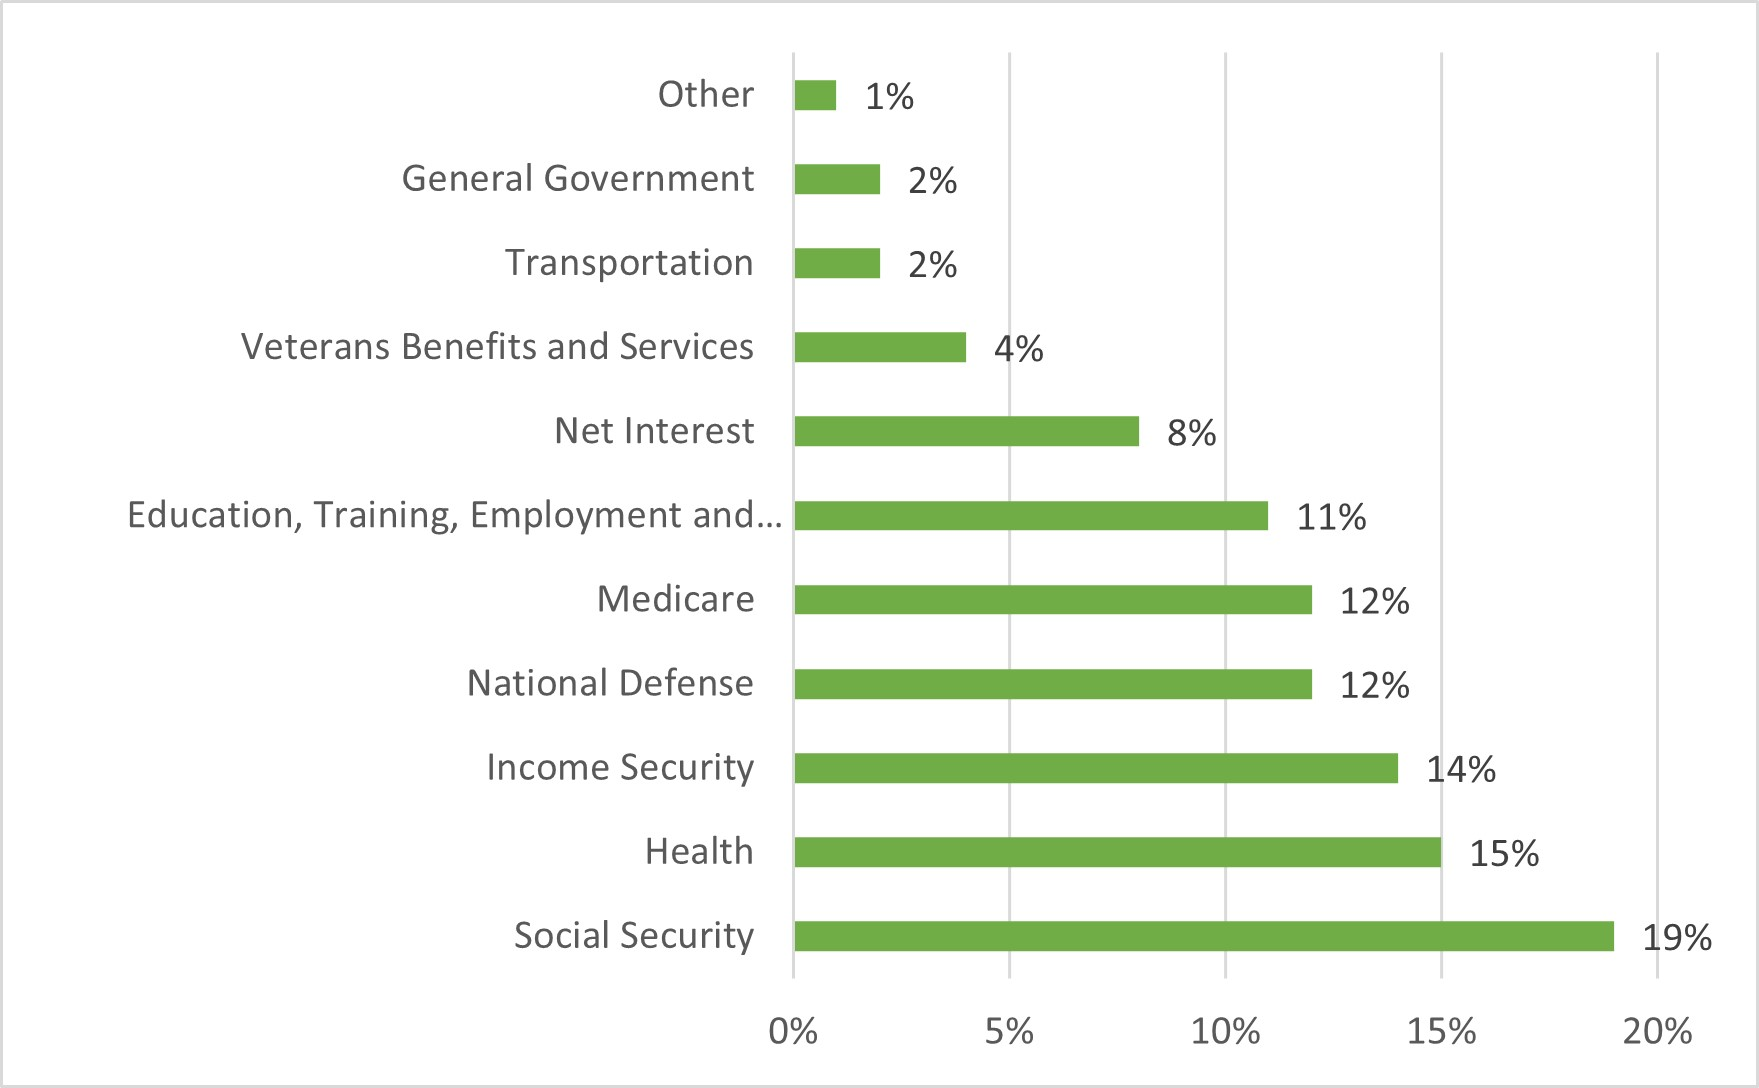
\includegraphics[scale=0.52]{Chapter-1/Figures/federal expenditure.JPG}  %以pic.jpg的0.5倍大小输出
        \end{minipage}
    }
    \subfigure[State and Local Expenditure]{ %second subfigure
        \begin{minipage}{7cm}
            \centering    %子图居中
            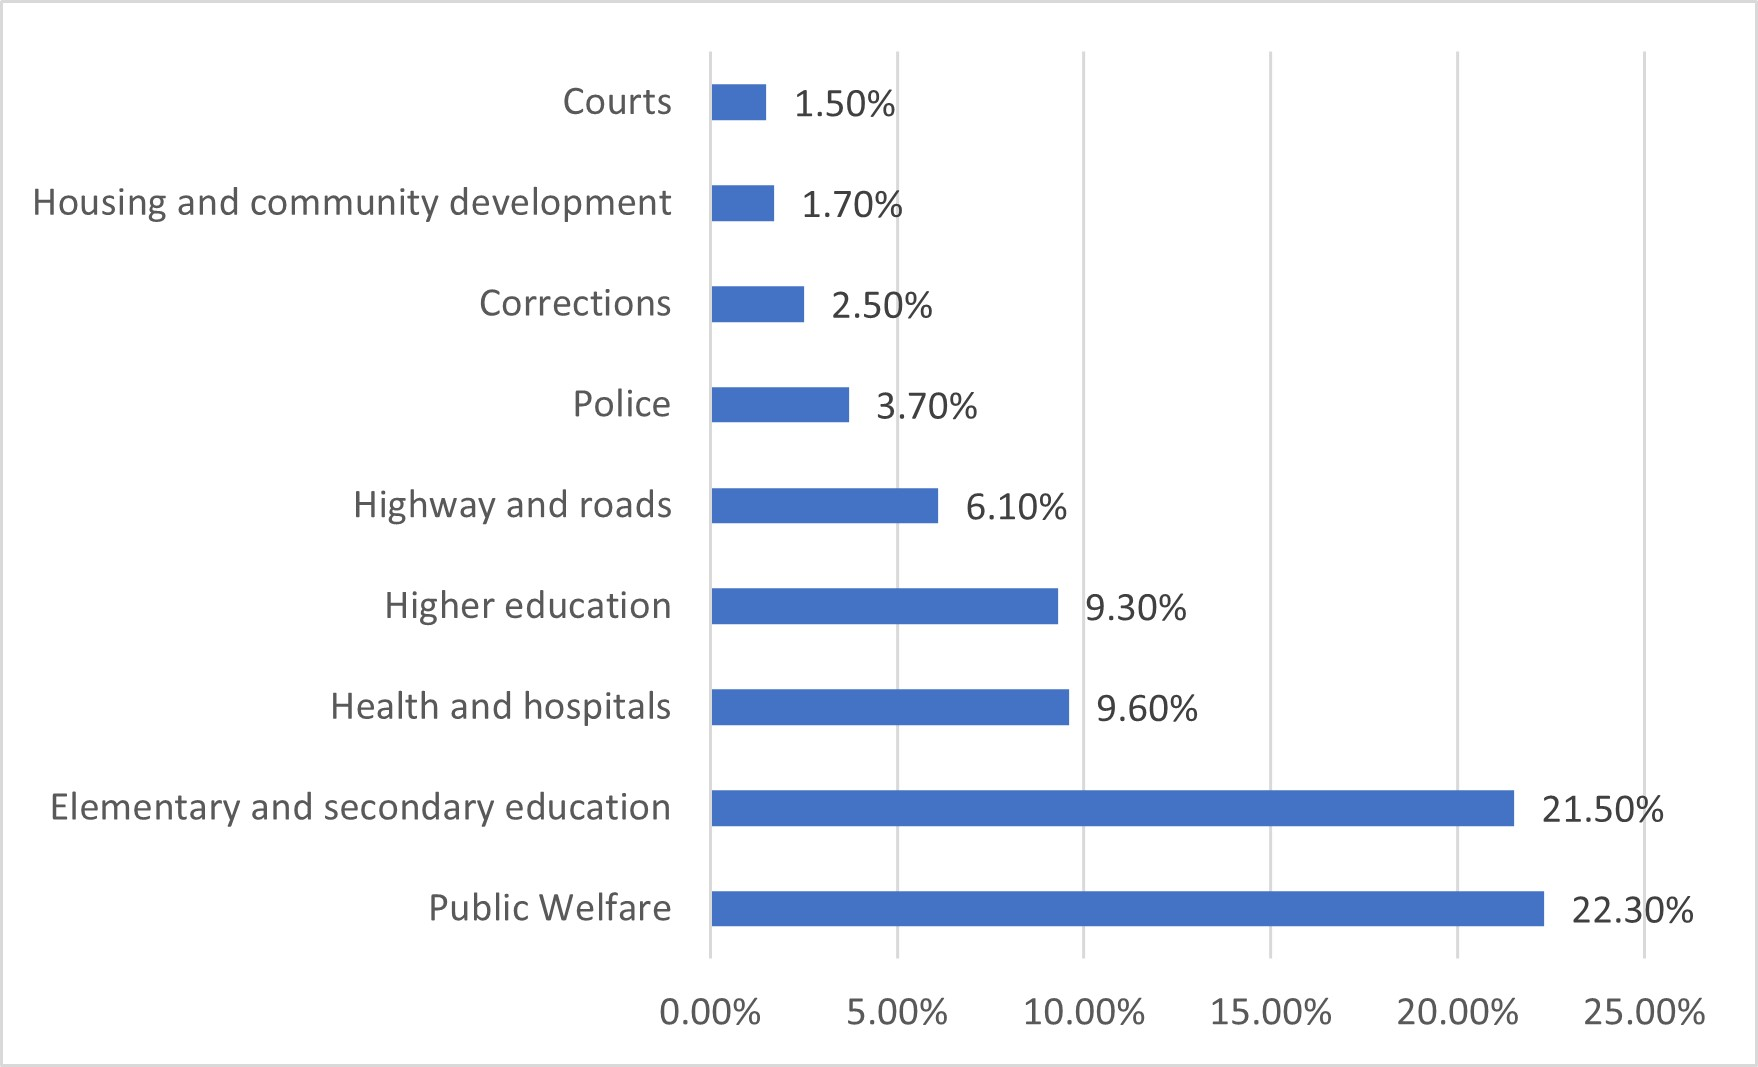
\includegraphics[scale=0.52]{Chapter-1/Figures/state and local expenditure.JPG}%以pic.jpg的0.5倍大小输出
        \end{minipage}
    }

    \caption[Expenditure Structure for Multiple Level of Governments in 2019]{Expenditure Structure for Multiple Level of Governments.}    %caption for whole figure
    \label{Figure 1.3}
\end{figure}
\clearpage

\begin{figure}[H]
    \centering
    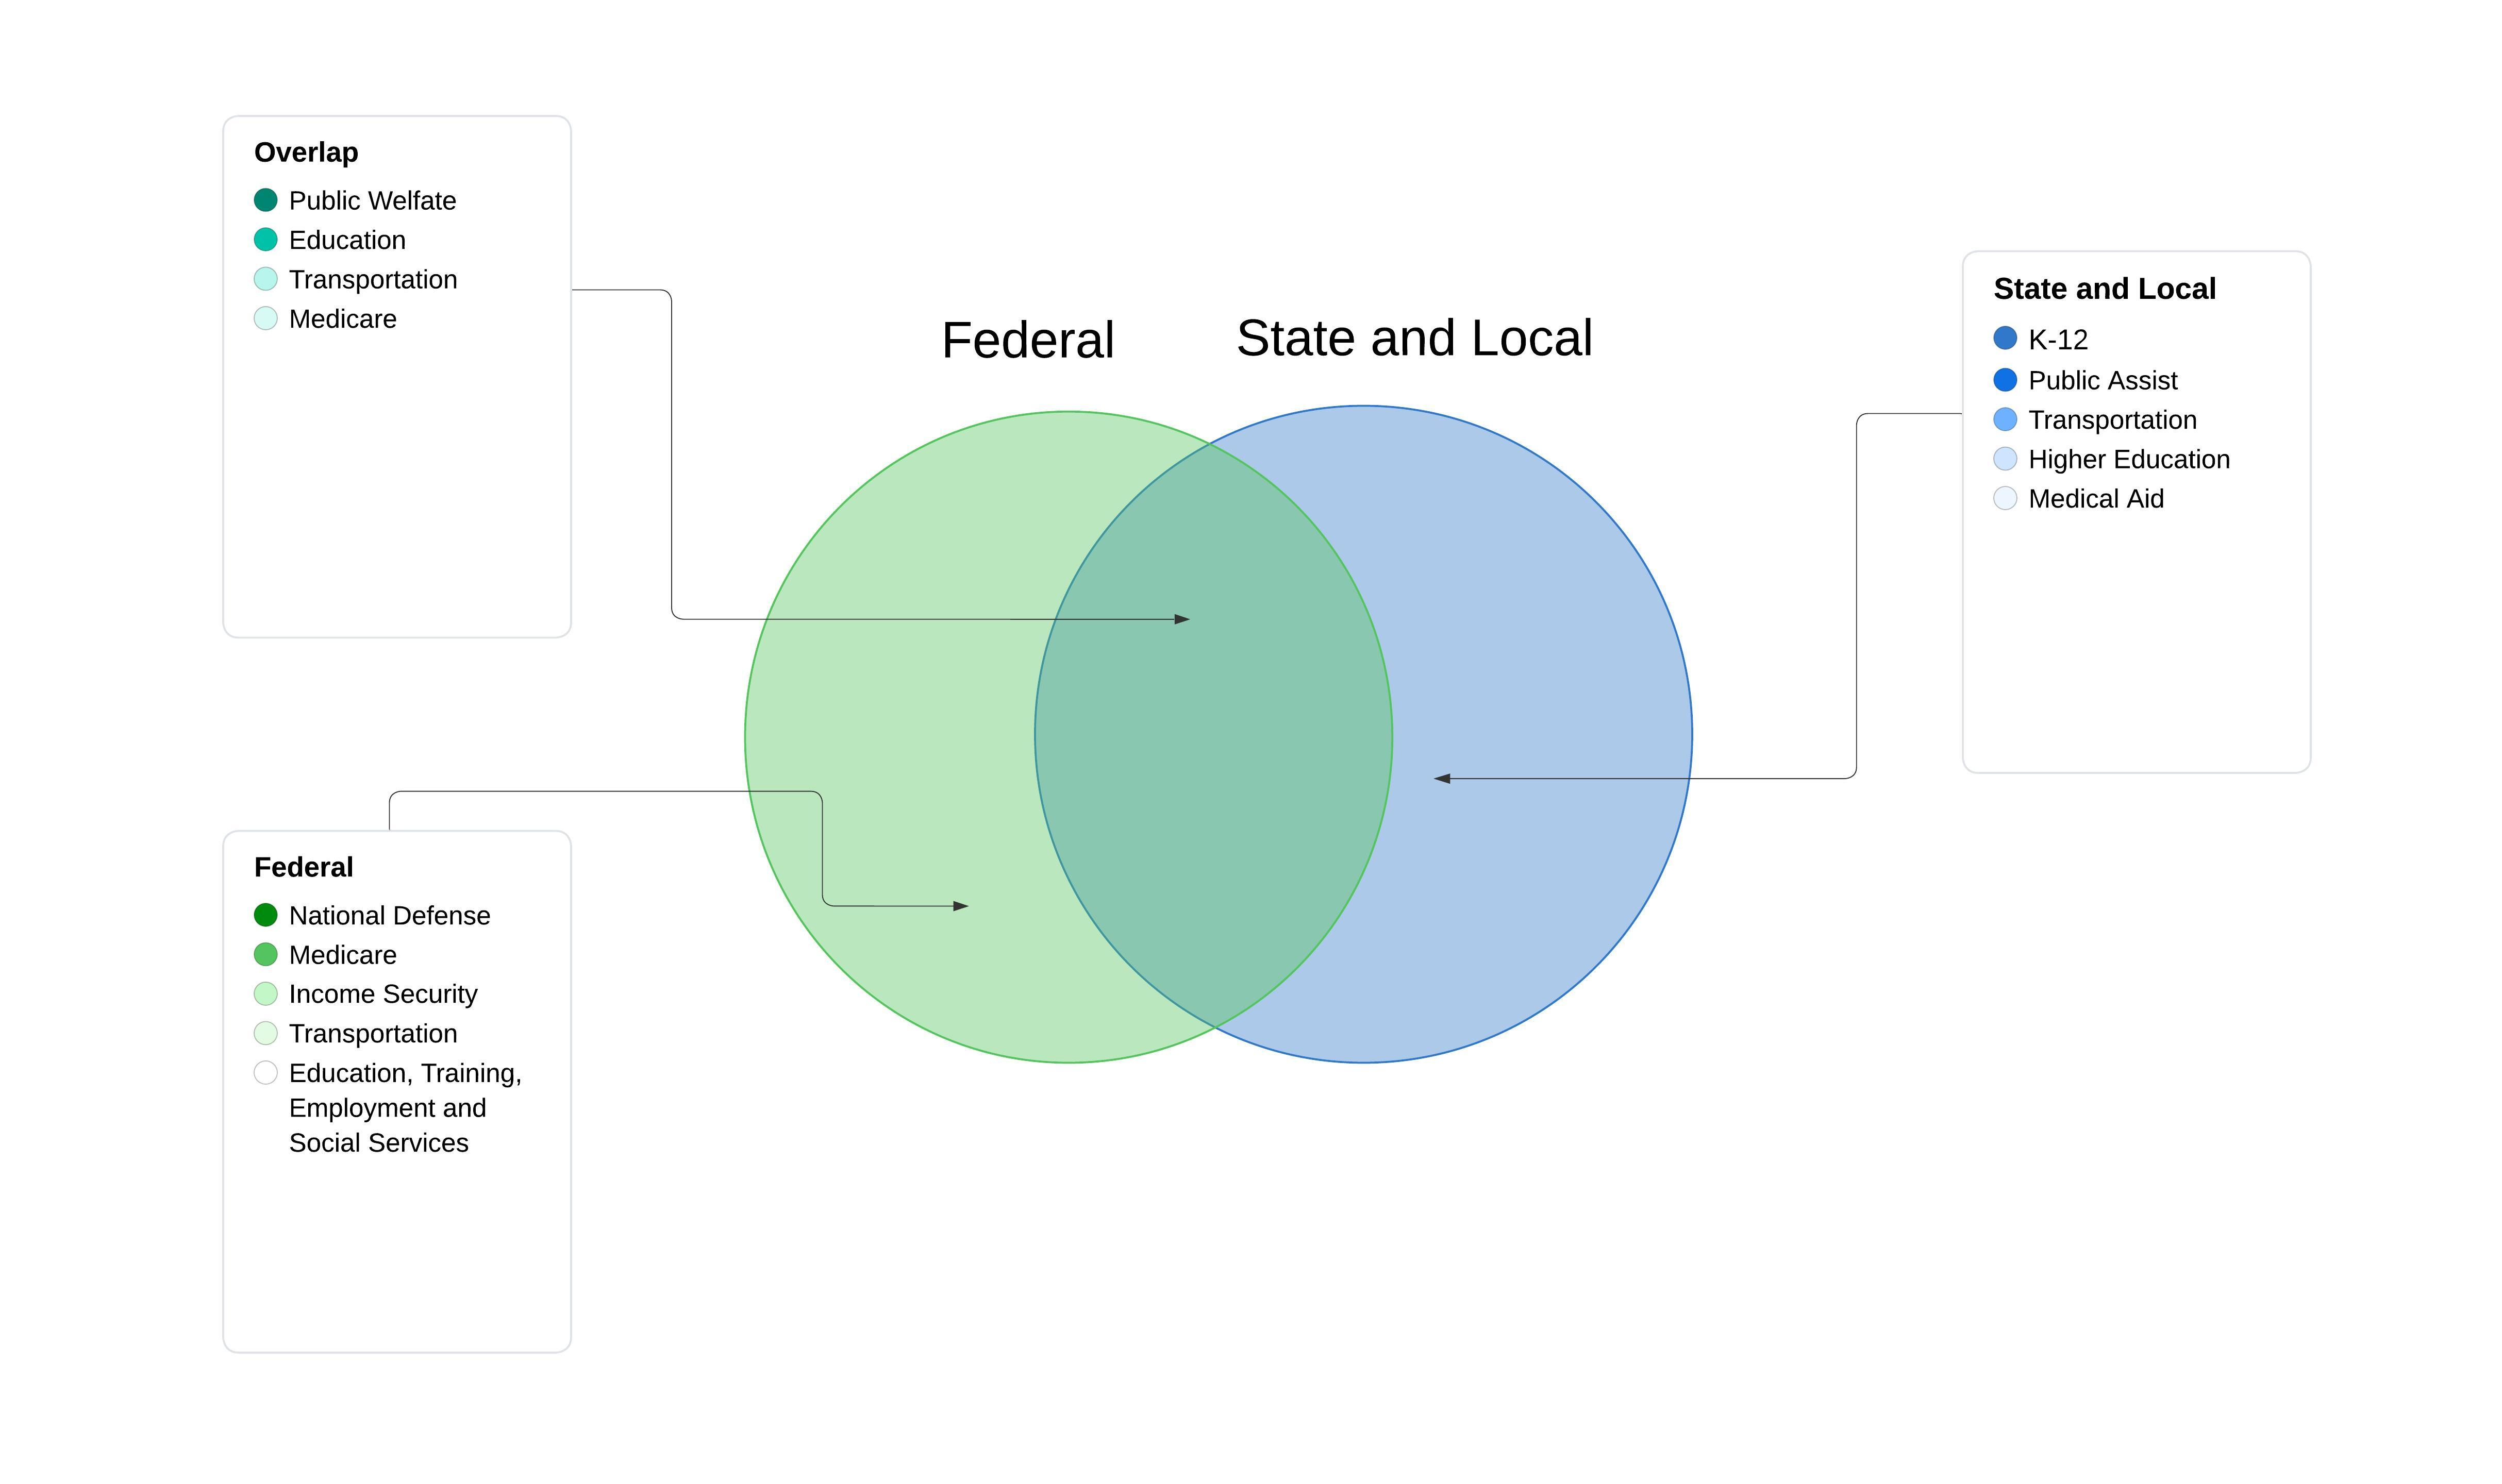
\includegraphics[scale=0.4]{Chapter-1/Figures/Venn graph on public goods.jpeg}
    \caption[Venn graph on public goods and services supplying]{Venn graph on public goods and services supplying by federal, states and local government
        \texttt{} }
    \label{Figure 1.4}
\end{figure}

\clearpage

\section{Chapter 2}

\begin{landscape}
    \begin{figure}[H]
        \centering
        \includegraphics[scale=0.045]{Chapter-2/Figures/tree.jpg}
        \caption[Dynamic Game Tree of 3 players]{Dynamic Game Tree between Central and Subnational Governments
            \texttt{} }
        \label{dynamicgamenoutility}
    \end{figure}
\end{landscape}
\newpage

\begin{figure}[htbp]
    \centering
    \subfigure[]{
        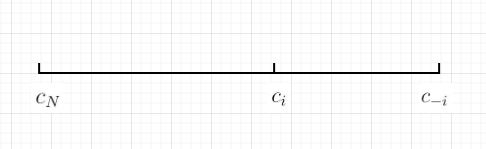
\includegraphics[width=0.61\textwidth]{Chapter-2/Figures/cncic-i.JPG}}
    \subfigure[]{
        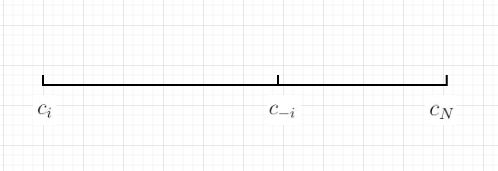
\includegraphics[width=0.61\textwidth]{Chapter-2/Figures/cic-icn.JPG}}
    \caption{When $c_N$ lies outside the range of $c_i$ and $c_{-i}$}
    \label{cnci}
\end{figure}

\begin{figure}[htbp]
    \centering
    \subfigure[]{
        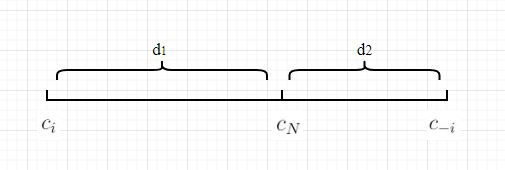
\includegraphics[width=0.71\textwidth]{Chapter-2/Figures/cicnc-i.JPG}}
    \subfigure[]{
        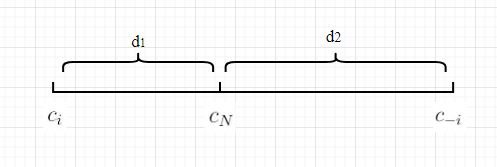
\includegraphics[width=0.71\textwidth]{Chapter-2/Figures/cicnc-i2.JPG}}
    \caption{When $c_N$ lies between $c_i$ and $c_i$}
    \label{cnci2}
\end{figure}
\clearpage
\section{Chapter 3}
\begin{figure}[H]
    \centering
    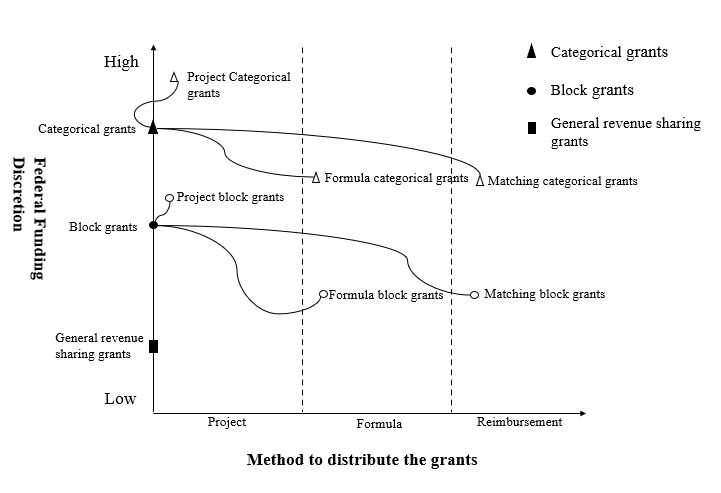
\includegraphics[scale=0.8]{Chapter-3/Figures/grants type.JPG}
    \caption[Grants Type in America]{Grants Type in America
        \texttt{} }
    \label{grantstype}
\end{figure}

% \begin{figure}[H]
%     \centering
%     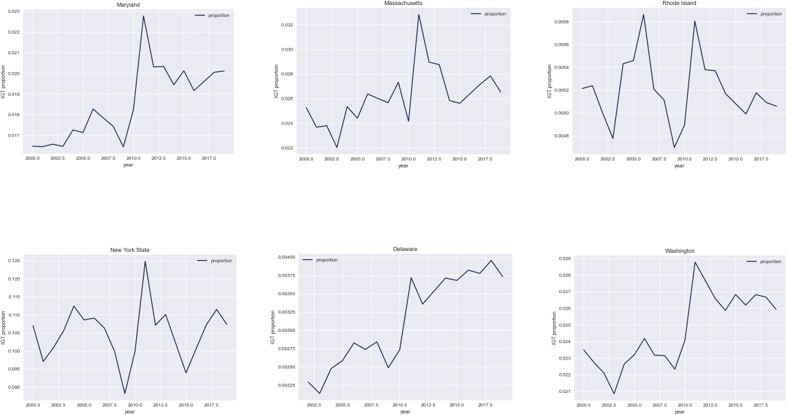
\includegraphics[scale=0.7]{Appendix-A/democratic.jpg}
%     \caption[Time Series Graph of Democratic States IGT(2000-2019)]{Time Series Graph of Democratic States IGT (2000-2019)
%         \texttt{} }
%     \label{Figure A.3}
% \end{figure}

% \begin{figure}[H]
%     \centering
%     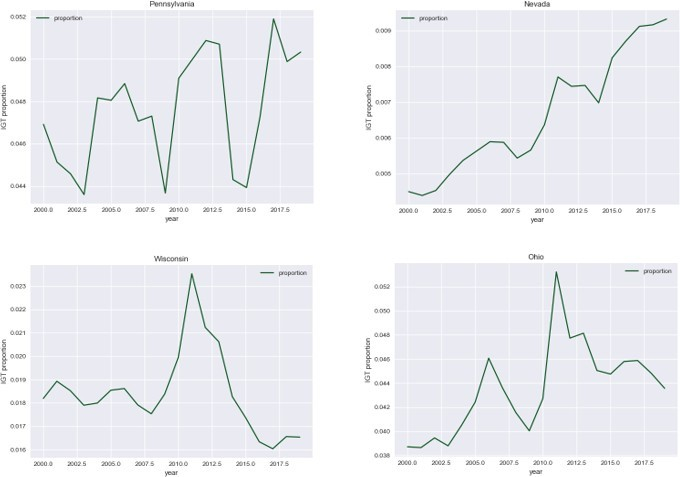
\includegraphics[scale=0.7]{Appendix-A/swing.jpg}
%     \caption[Time Series Graph of Swing States IGT (2000-2019) ]{Time Series Graph of Swing States IGT (2000-2019)
%         \texttt{} }
%     \label{Figure A.4}
% \end{figure}

\clearpage
\begin{figure}[H]
    \centering
    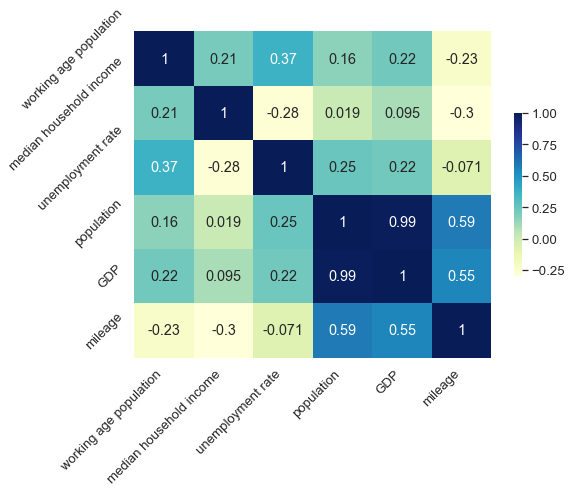
\includegraphics[scale=0.7]{Chapter-3/Figures/heatmap.png}
    \caption[Heatmap of the Social Characteristics]{Heatmap of the Social Characteristics
        \texttt{} }
    \label{heatmap}
\end{figure}
\clearpage

\begin{figure}[H]
    \centering  %居中
    \subfigure[Histgram]{   %第一张子图
        \begin{minipage}{7cm}
            \centering    %子图居中
            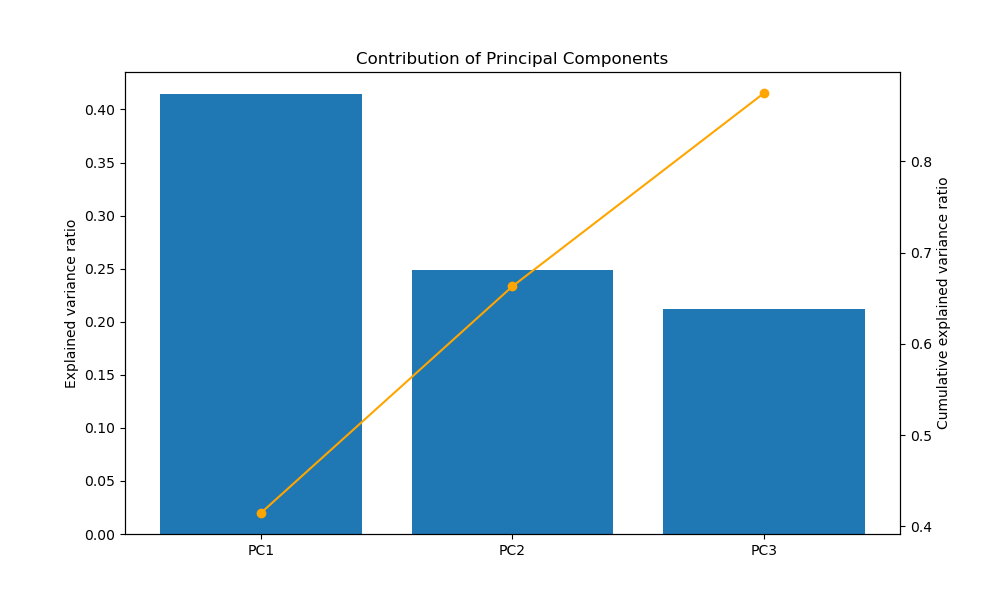
\includegraphics[scale=0.2]{Chapter-3/Figures/contribution.png}  %以pic.jpg的0.5倍大小输出
        \end{minipage}
    }
    \subfigure[Line]{ %第二张子图
        \begin{minipage}{7cm}
            \centering    %子图居中
            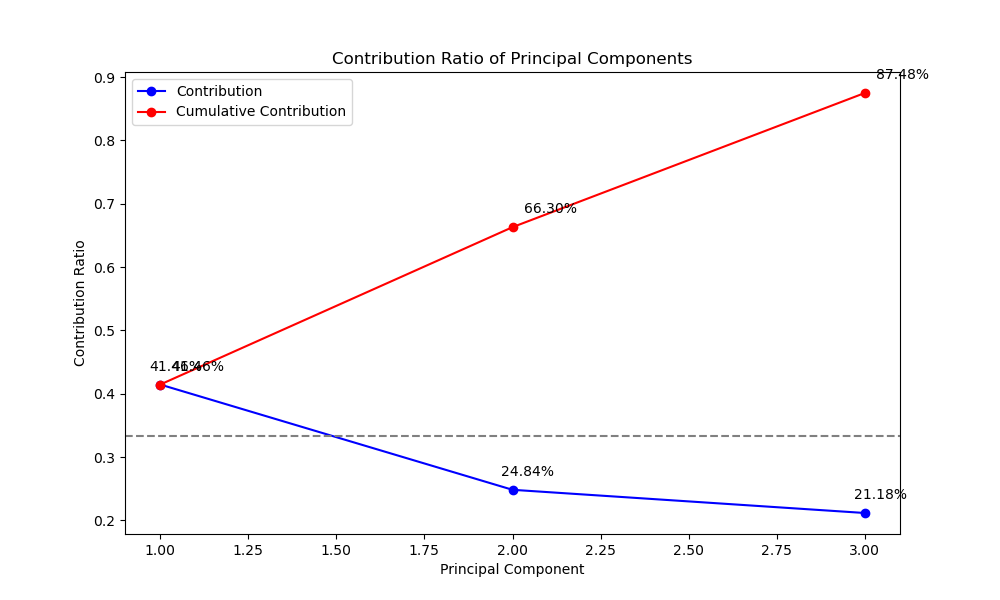
\includegraphics[scale=0.2]{Chapter-3/Figures/contribution2.png}%以pic.jpg的0.5倍大小输出
        \end{minipage}
    }
    \caption[Principle Components Contribution]{Principle Components Contribution}    %大图名称
    \label{principlecomponentcontribution}    %图片引用标记
\end{figure}
\clearpage


\begin{figure}[H]
    \centering  %居中
    \subfigure[2 Principle Components Analysis Scatter]{   %第一张子图
        \begin{minipage}{7cm}
            \centering    %子图居中
            \includegraphics[scale=0.45]{Chapter-3/Figures/pca.png}  %以pic.jpg的0.5倍大小输出
        \end{minipage}
    }
    \subfigure[3 principle Components Analysis Scatter]{ %第二张子图
        \begin{minipage}{7cm}
            \centering    %子图居中
            \includegraphics[scale=0.45]{Chapter-3/Figures/pca_3d.png}%以pic.jpg的0.5倍大小输出
        \end{minipage}
    }
    \caption[Principle Components Analysis Scatter Plot]{Social Characteristics Principle Components Analysis Scatter Plot}    %大图名称
    \label{Figure 2.2}    %图片引用标记
\end{figure}
\clearpage
\begin{figure}[H]
    \centering
    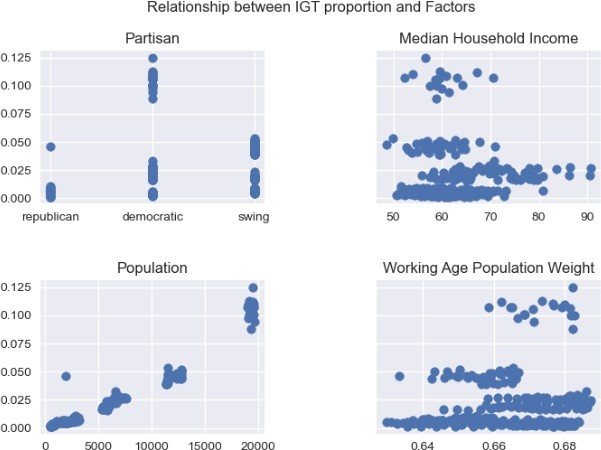
\includegraphics[scale=1]{Chapter-3/Figures/IGT and factors.jpg}
    \caption[IGT and Factors Scatter Plot]{Factor and IGT Scatter Plot
        \texttt{} }
    \label{Figure 2.3}
\end{figure}

\clearpage

\section{Chapter 4}

\begin{figure}[H]
    \centering
    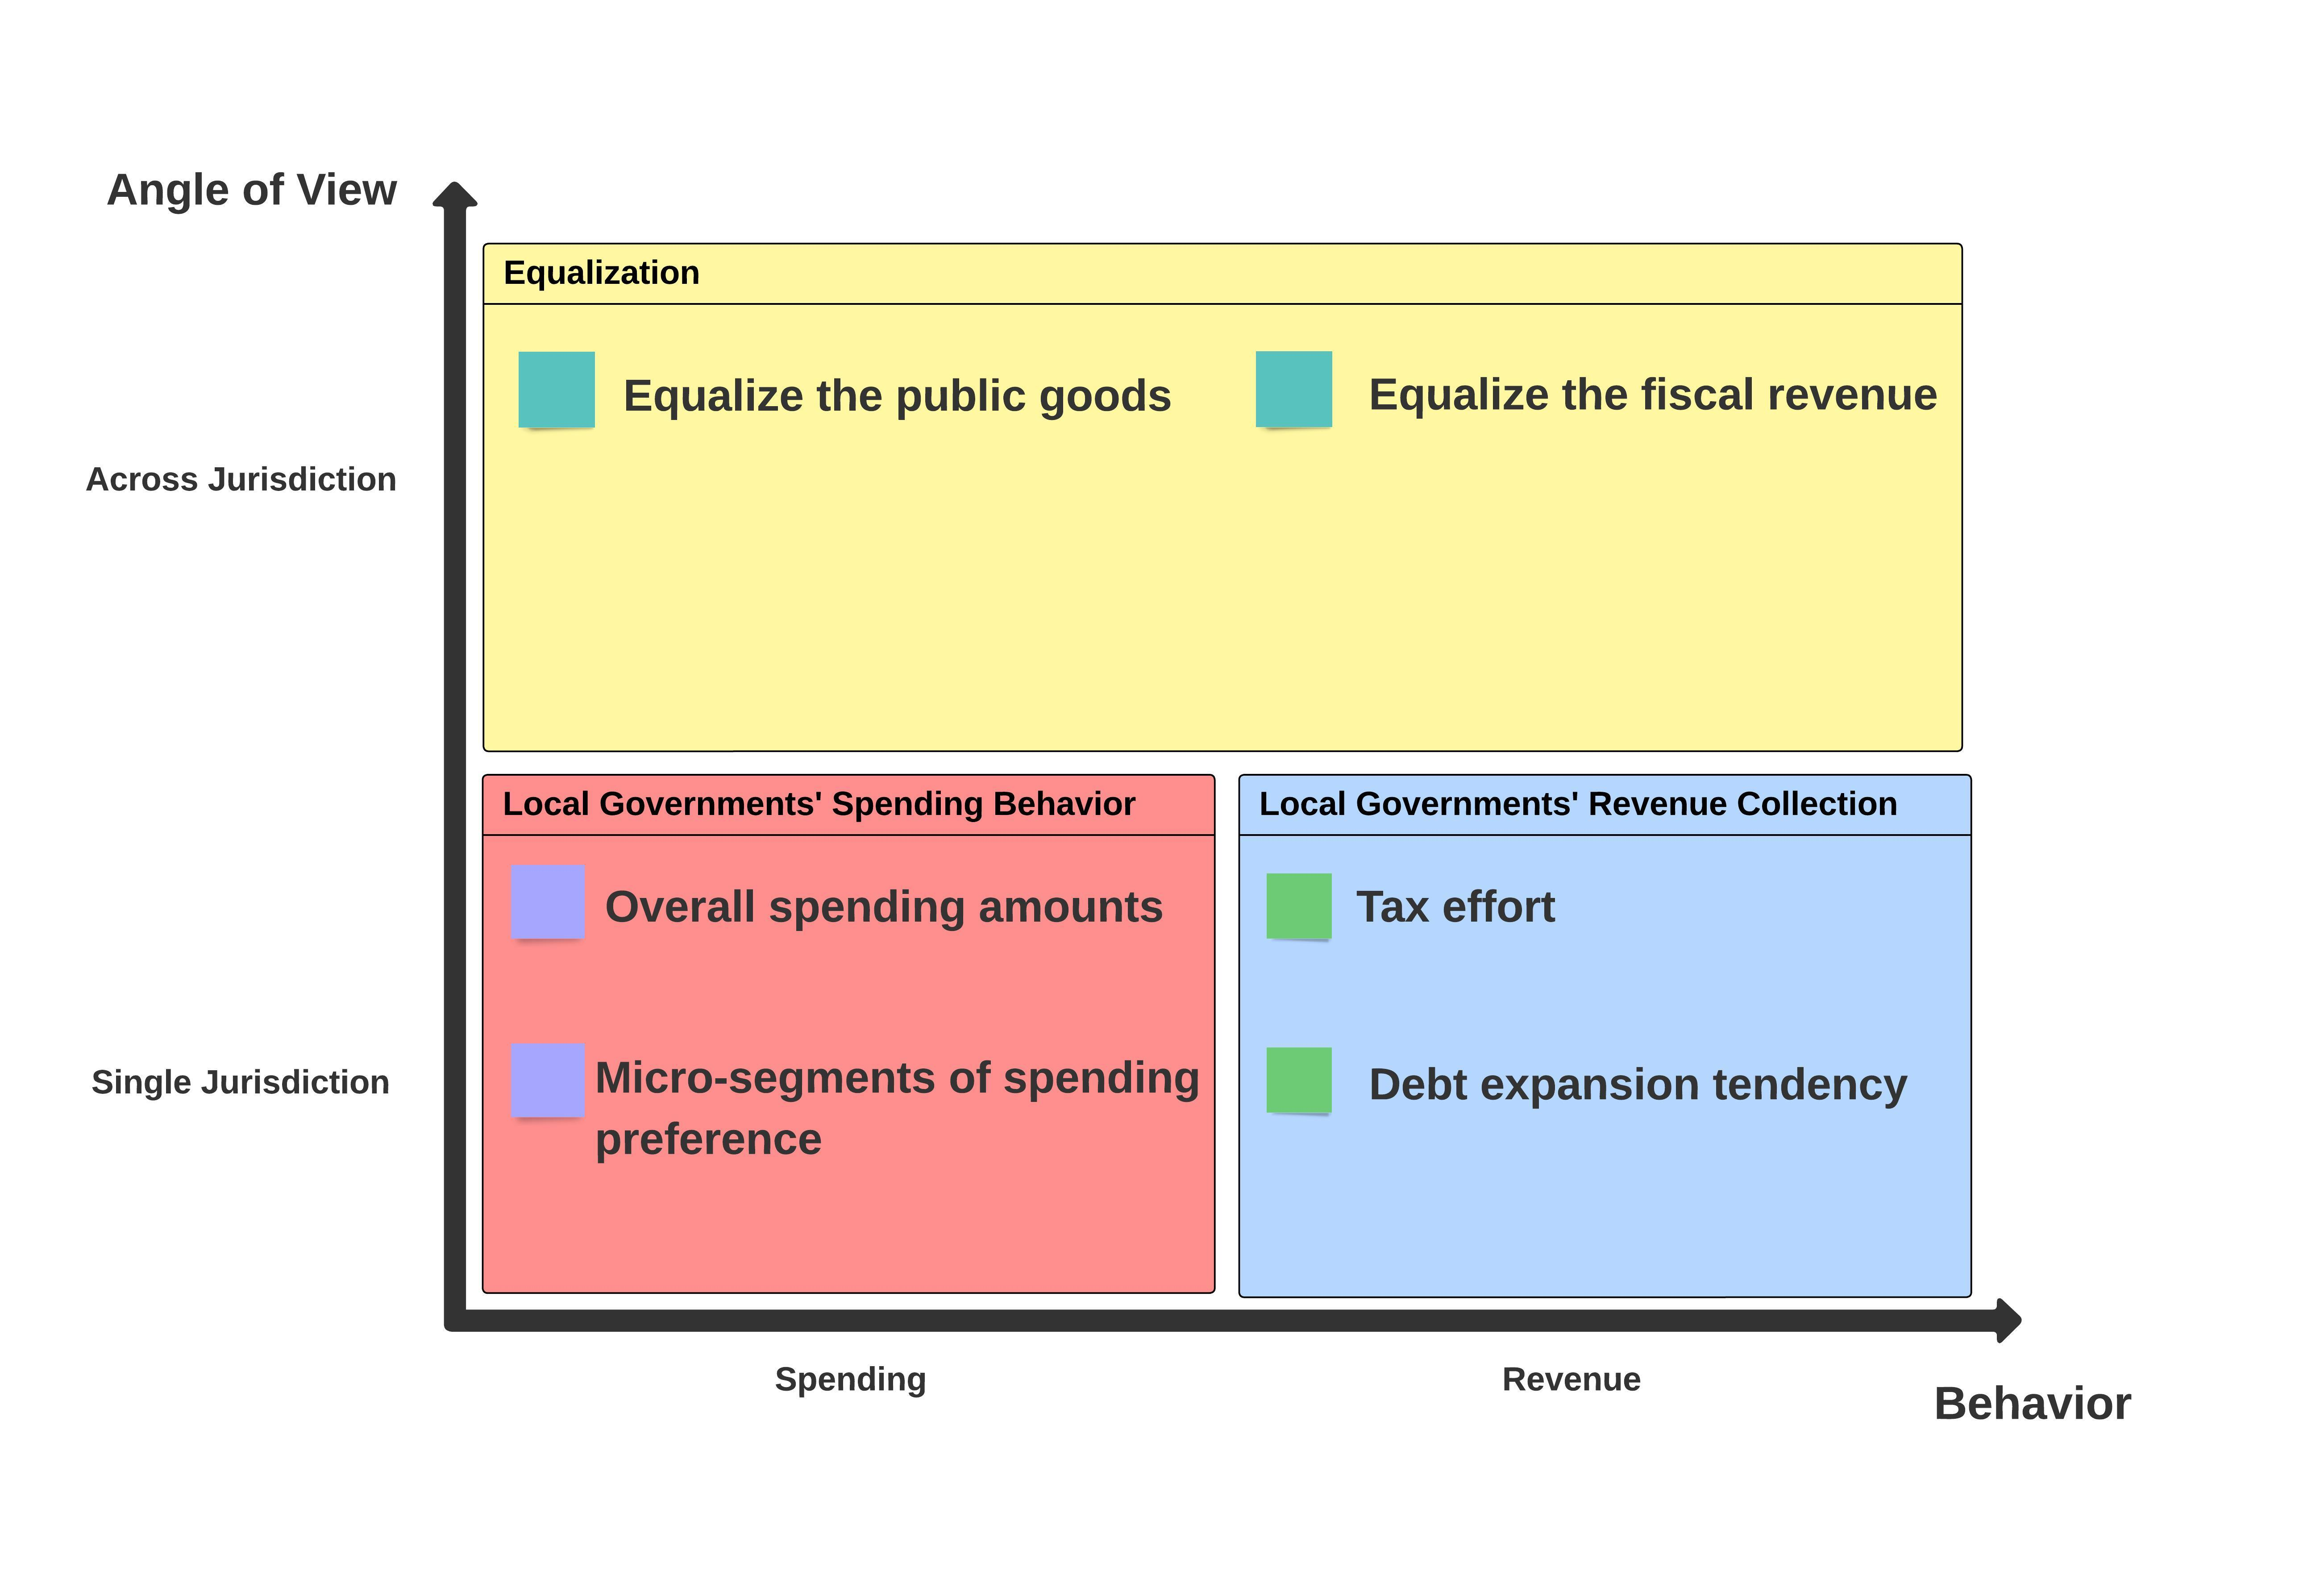
\includegraphics[scale=0.4]{Chapter-4/Figures/Effect of Intergovernmental Transfer.jpeg}
    \caption{Effect of Intergovernmental Transfer
        \texttt{} }
    \label{Figure 3.1}
\end{figure}
\clearpage
\begin{figure}[H]
    \centering
    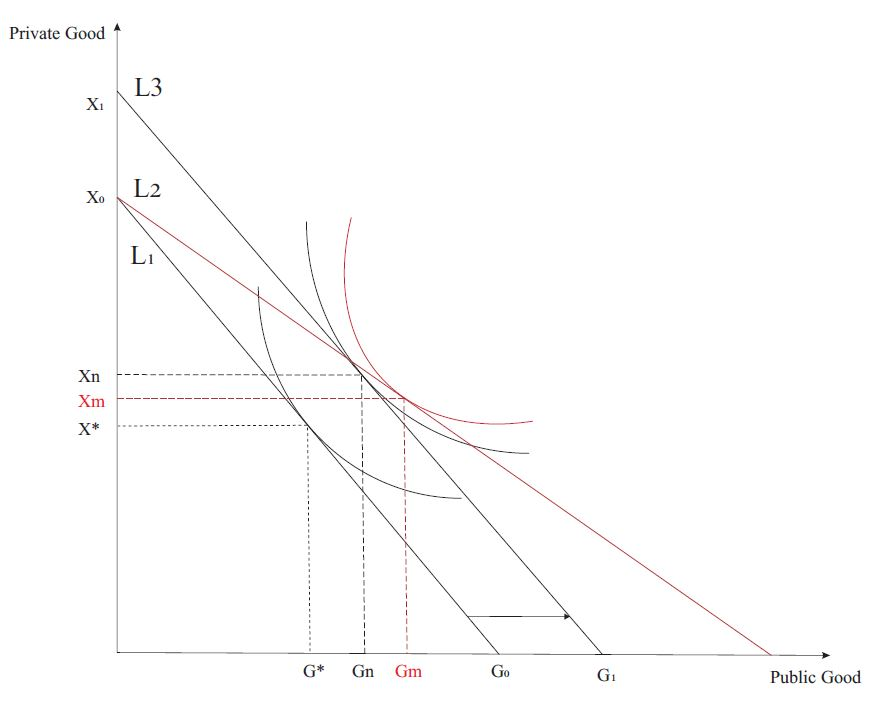
\includegraphics[scale=0.4]{Chapter-4/Figures/mfyeffect.jpg}
    \caption[Income Effect and Price Effect of Matching and Non-matching Grants]{Income Effect and Price Effect of Matching and Non-matching Grants
        \texttt{} }
    \label{Figure 3.3}
\end{figure}

\clearpage

\begin{figure}[H]
    \centering
    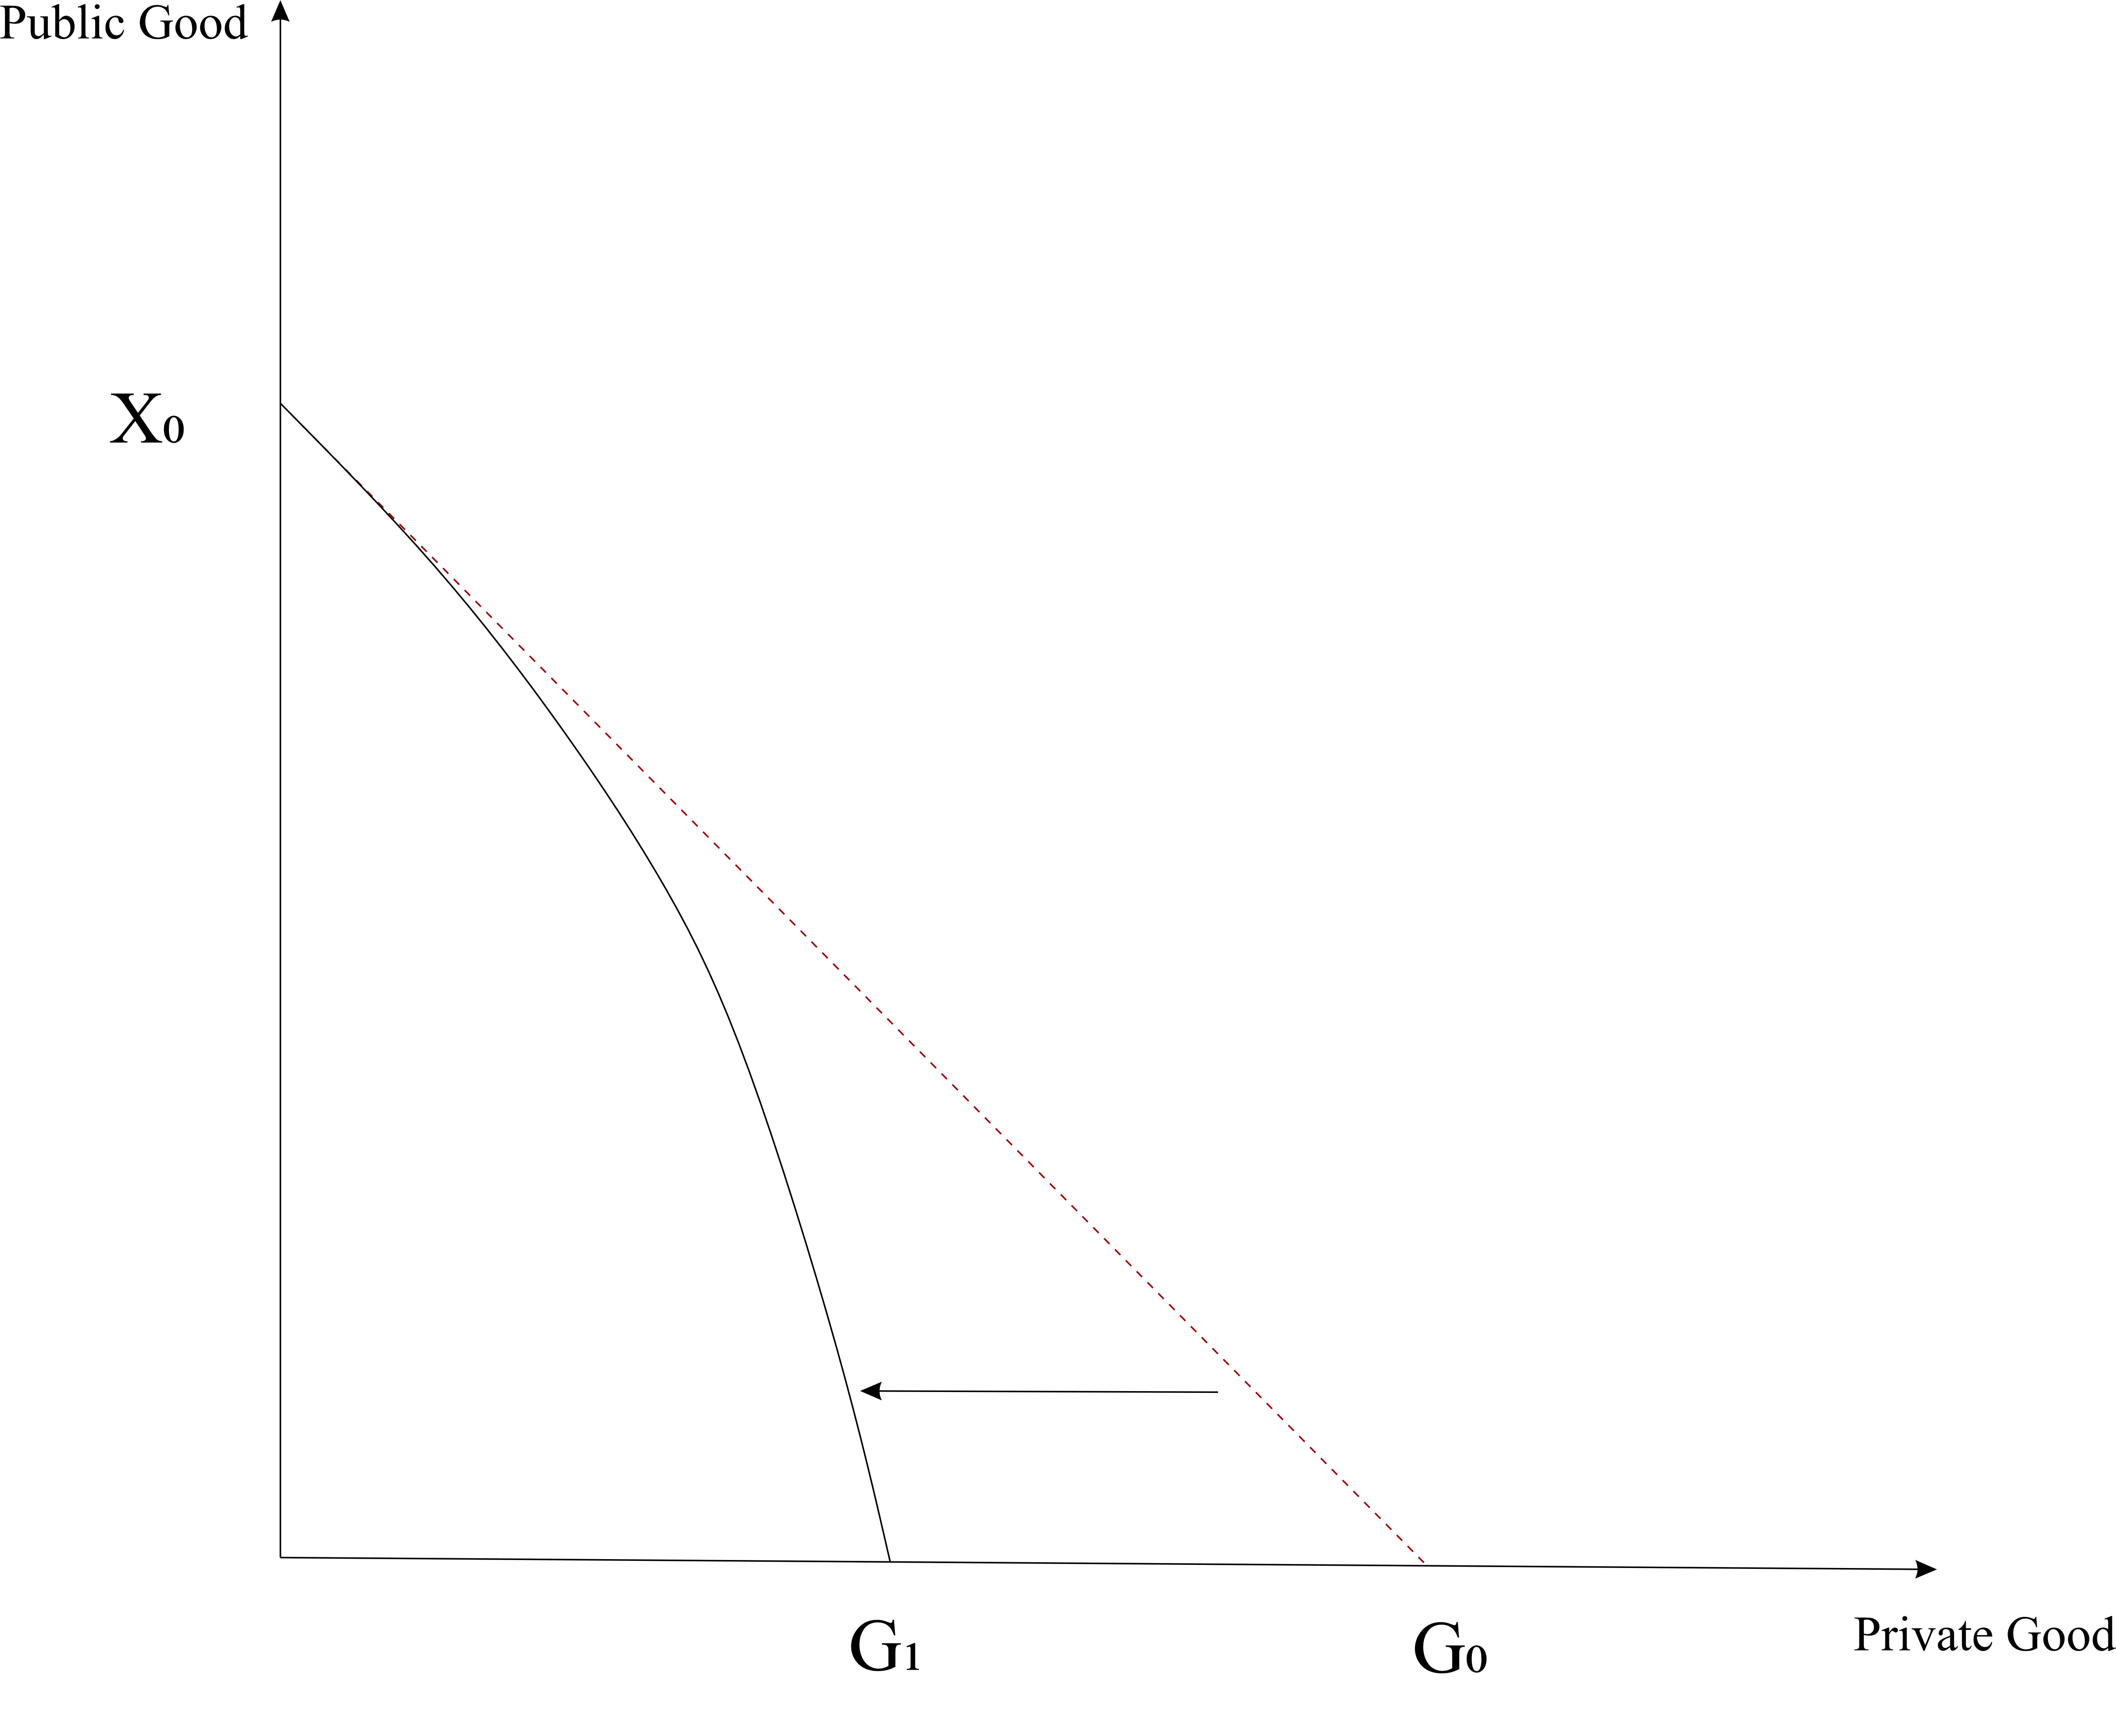
\includegraphics[scale=0.4]{Chapter-4/Figures/budget constrain distortion.jpg}
    \caption[Hamilton's Curved Budget Constraint]{Hamilton's Curved Budget Constrain
        \texttt{} }
    \label{Figure 3.4}
\end{figure}

\clearpage

\begin{figure}[htbp]
    \centering
    \subfigure[]{
        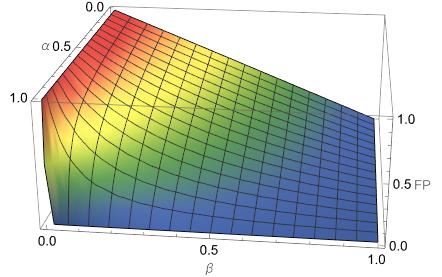
\includegraphics[width=0.45\textwidth]{Chapter-4/Figures/distofp1.jpg}}
    \subfigure[]{
        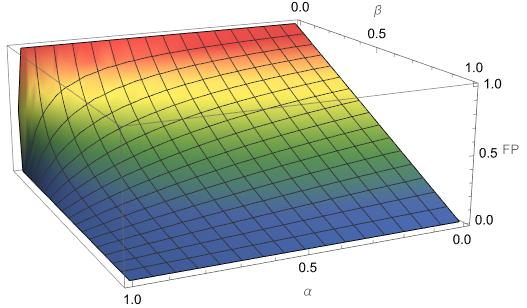
\includegraphics[width=0.45\textwidth]{Chapter-4/Figures/distofp2.jpg}}
    \subfigure[]{
        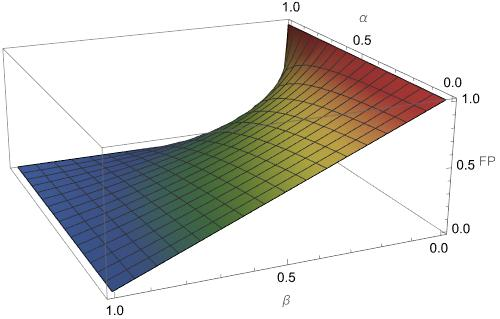
\includegraphics[width=0.45\textwidth]{Chapter-4/Figures/distofp3.jpg}}
    \subfigure[]{
        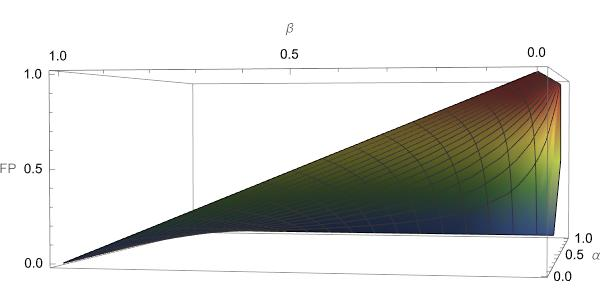
\includegraphics[width=0.45\textwidth]{Chapter-4/Figures/distofp4.jpg}}
    \caption{3-Dimensions Plot of the Fluctuation of Flypaper Effect under Distortion}
    \label{figfeunderdistortion}
\end{figure}

\clearpage

\begin{figure}[H]
    \centering
    \subfigure[$\beta=0.1$]{
        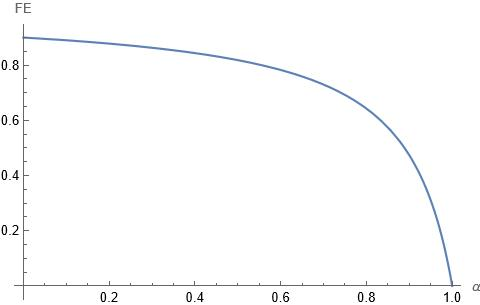
\includegraphics[width=0.45\textwidth]{Chapter-4/Figures/beta01.jpg}}
    \subfigure[$\beta=0.4$]{
        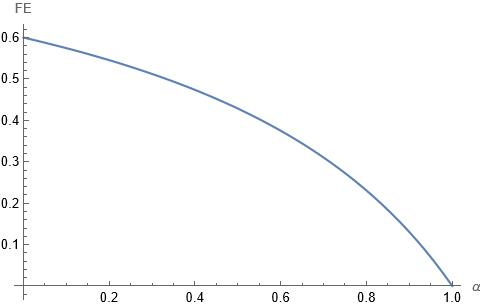
\includegraphics[width=0.45\textwidth]{Chapter-4/Figures/beta04.jpg}}
    \subfigure[$\beta=0.7$]{
        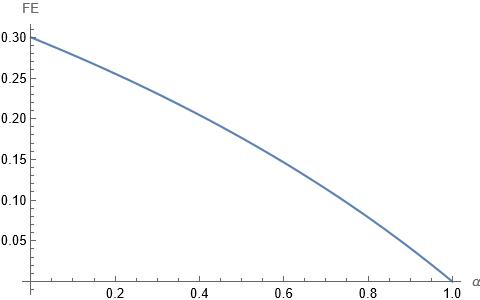
\includegraphics[width=0.45\textwidth]{Chapter-4/Figures/beta07.jpg}}
    \subfigure[$\beta=0.9$]{
        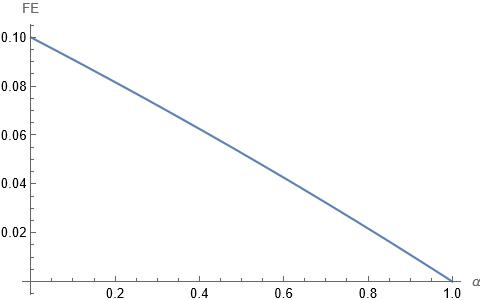
\includegraphics[width=0.45\textwidth]{Chapter-4/Figures/beta09.jpg}}
    \caption{2-Dimensions Plot of the Fluctuation of Flypaper Effect on $\alpha$}
    \label{fealpha}
\end{figure}
\clearpage
\begin{figure}[H]
    \centering
    \subfigure[$\alpha=0.1$]{
        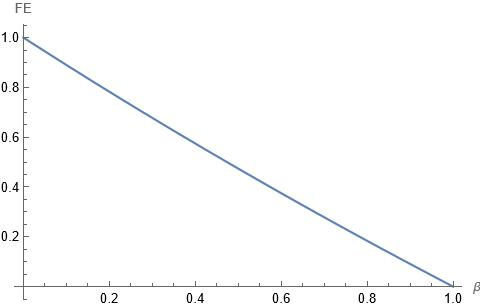
\includegraphics[width=0.45\textwidth]{Chapter-4/Figures/alpha01.jpg}}
    \subfigure[$\alpha=0.4$]{
        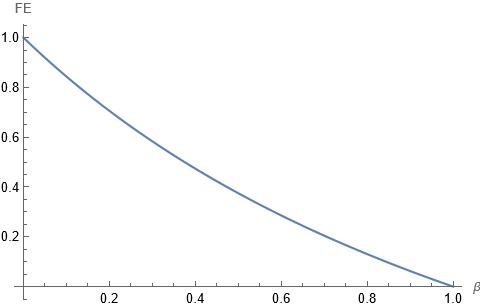
\includegraphics[width=0.45\textwidth]{Chapter-4/Figures/alpha04.jpg}}
    \subfigure[$\alpha=0.7$]{
        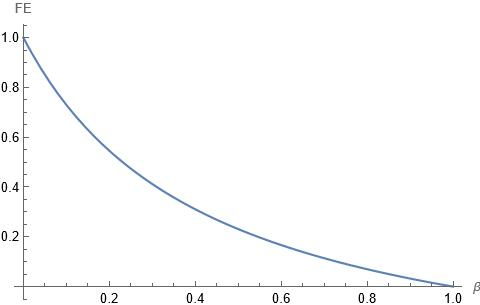
\includegraphics[width=0.45\textwidth]{Chapter-4/Figures/alpha07.jpg}}
    \subfigure[$\alpha=0.9$]{
        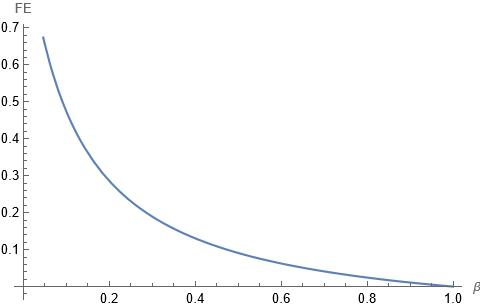
\includegraphics[width=0.45\textwidth]{Chapter-4/Figures/alpha09.jpg}}
    \caption{2-Dimensions Plot of the Fluctuation of Flypaper Effect on $\beta$}
    \label{febeta}
\end{figure}
\clearpage
\section{Chapter 5}

\begin{figure}[H]
    \centering
    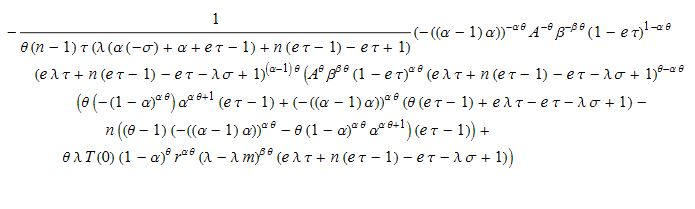
\includegraphics[scale=0.8]{Chapter-5/Figures/calculation effortttt.JPG}
    \caption[Expression of $\frac{\partial e_{i,t}}{\partial n}$]{Expression of $\frac{\partial e_{i,t}}{\partial n}$
        \texttt{} }
    \label{enenen}
\end{figure}

\clearpage

\begin{figure}[H]
    \centering
    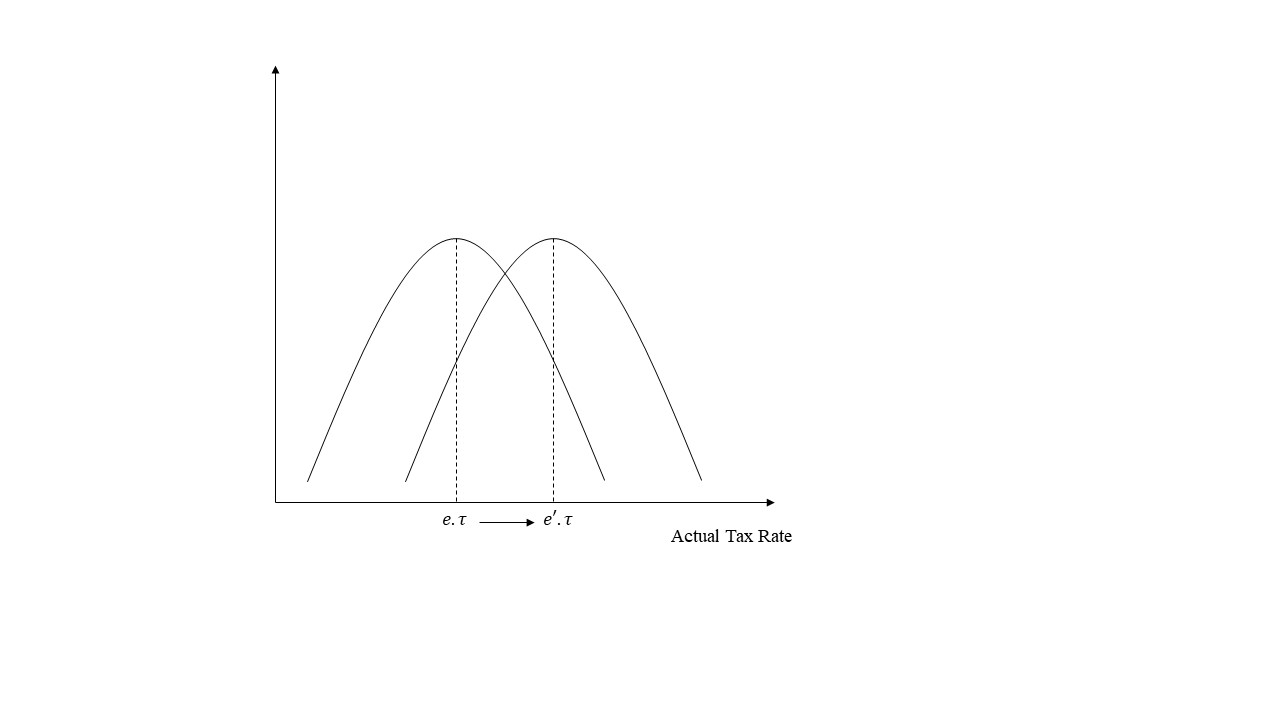
\includegraphics[scale=0.7]{Chapter-5/Figures/laffer.jpg}
    \caption[Laffer Curve for Tax Collection Effort]{Laffer Curve for Tax Collection Effort
        \texttt{} }
    \label{laffer}
\end{figure}

\clearpage
\begin{figure}[H]
    \centering
    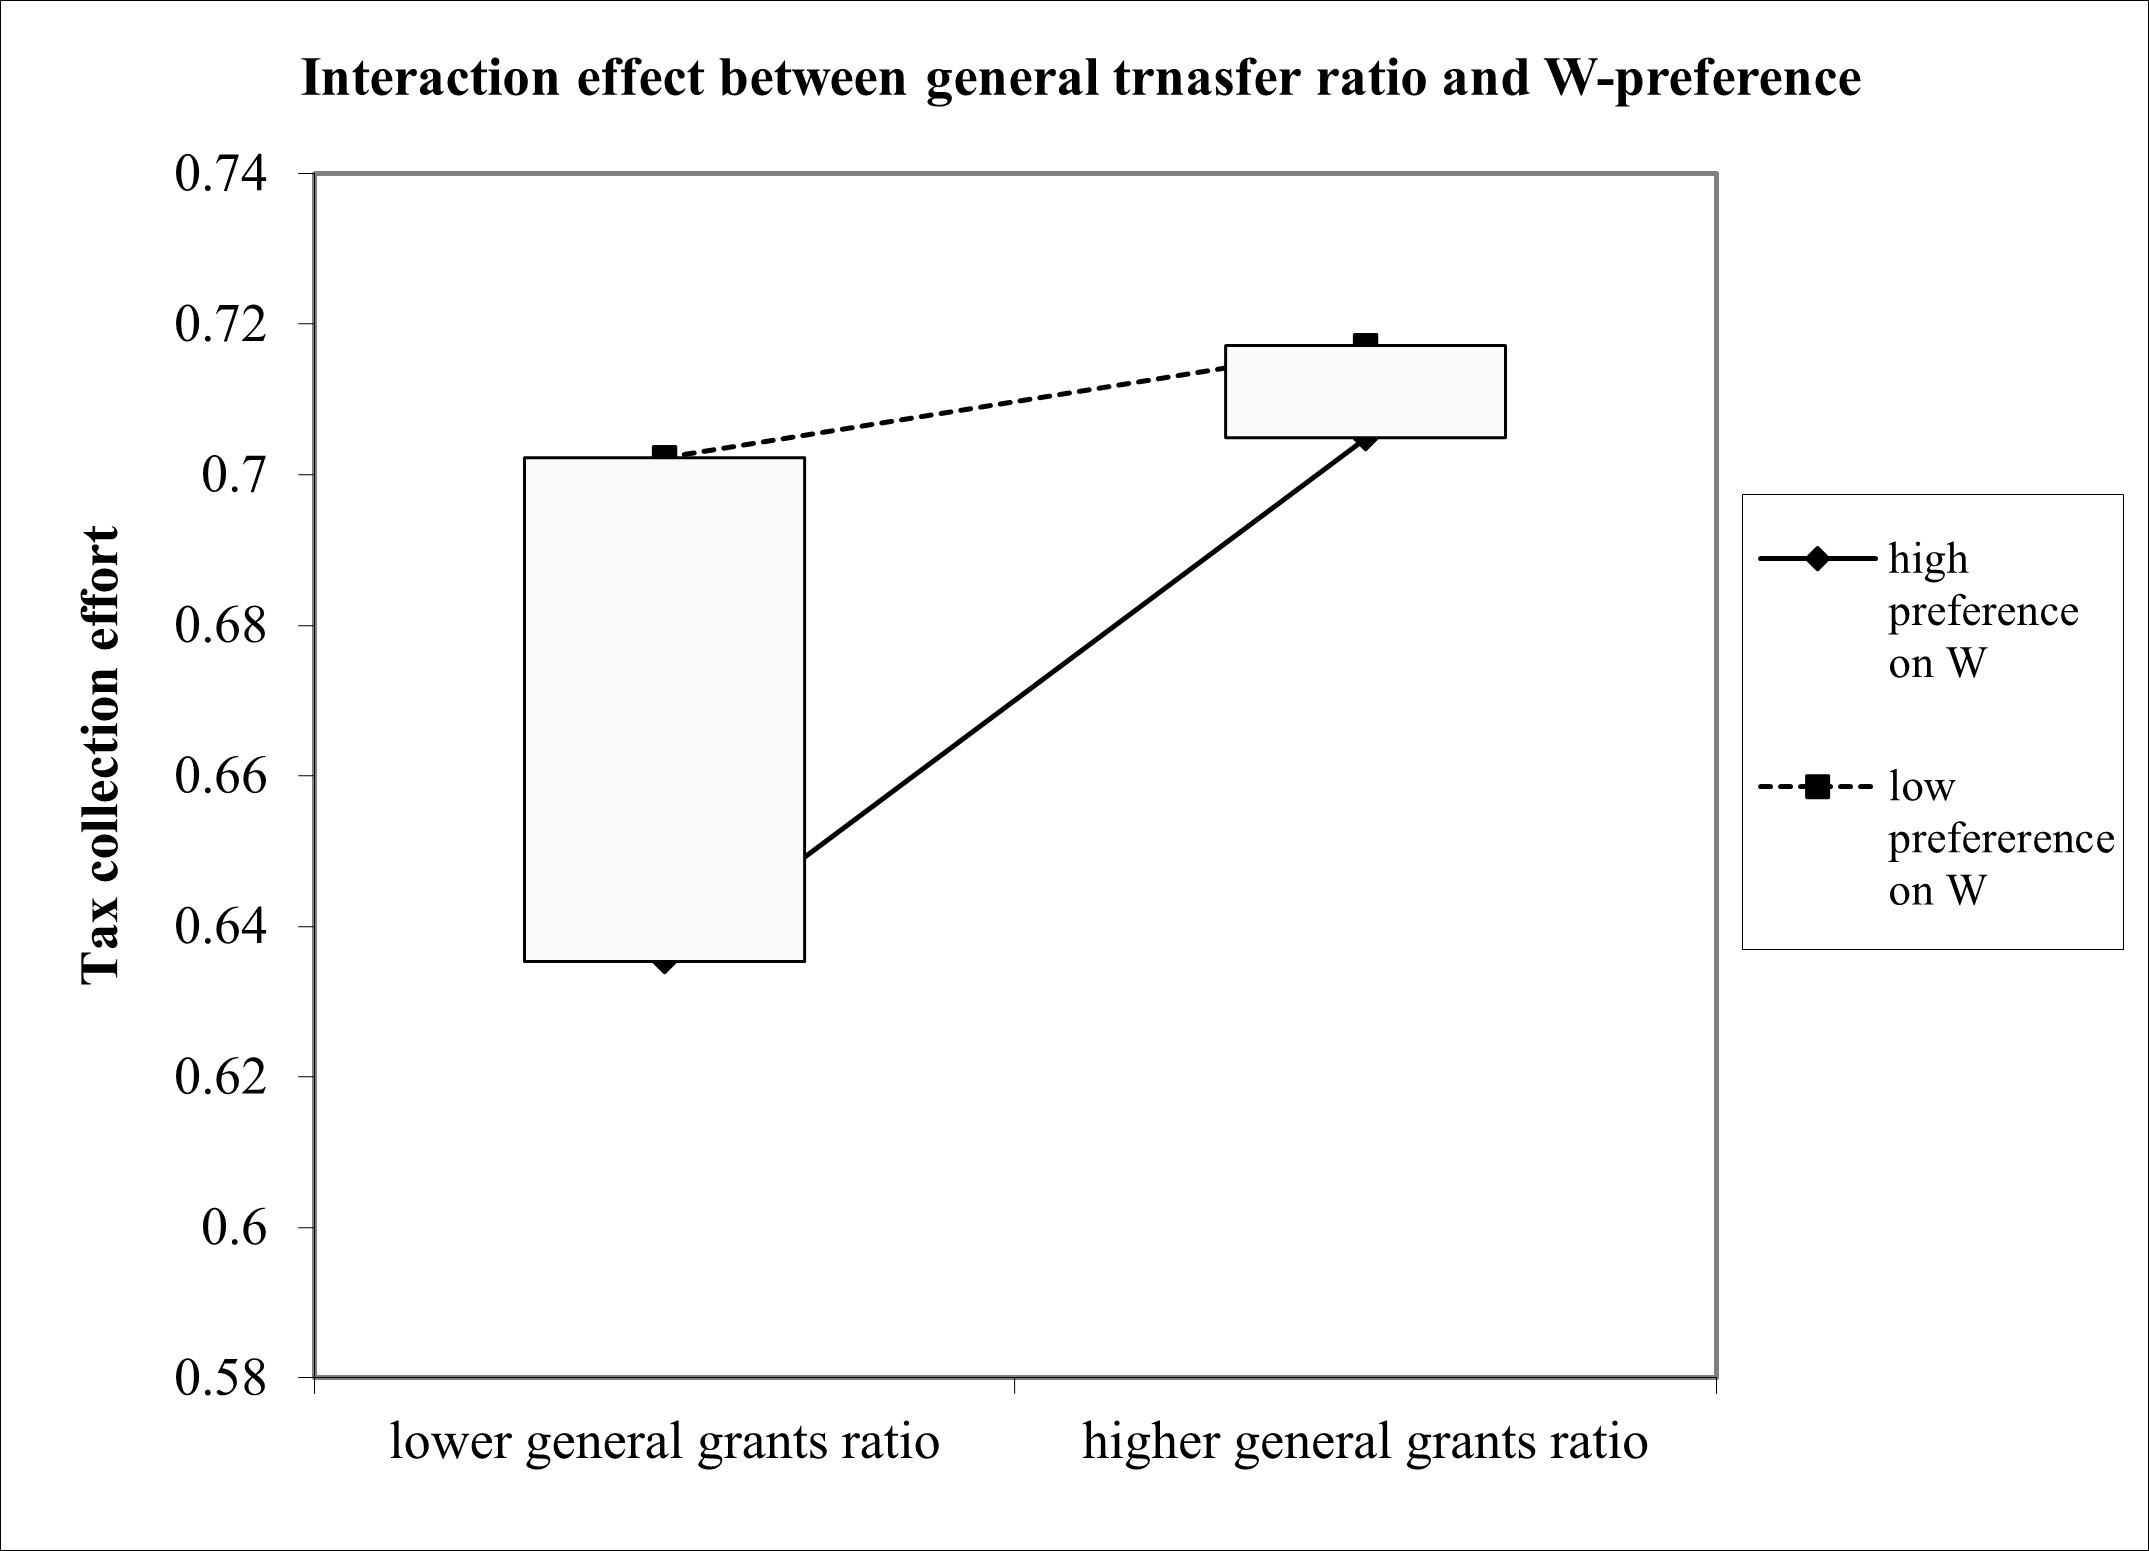
\includegraphics[scale=0.8]{Chapter-5/Figures/int_gen_W.jpg}
    \caption[Interaction effect between general transfer ratio and W-preference]{Interaction effect between general trnasfer ratio and W-preference
        \texttt{} }
    \label{int_gen_W}
\end{figure}

\begin{figure}[H]
    \centering
    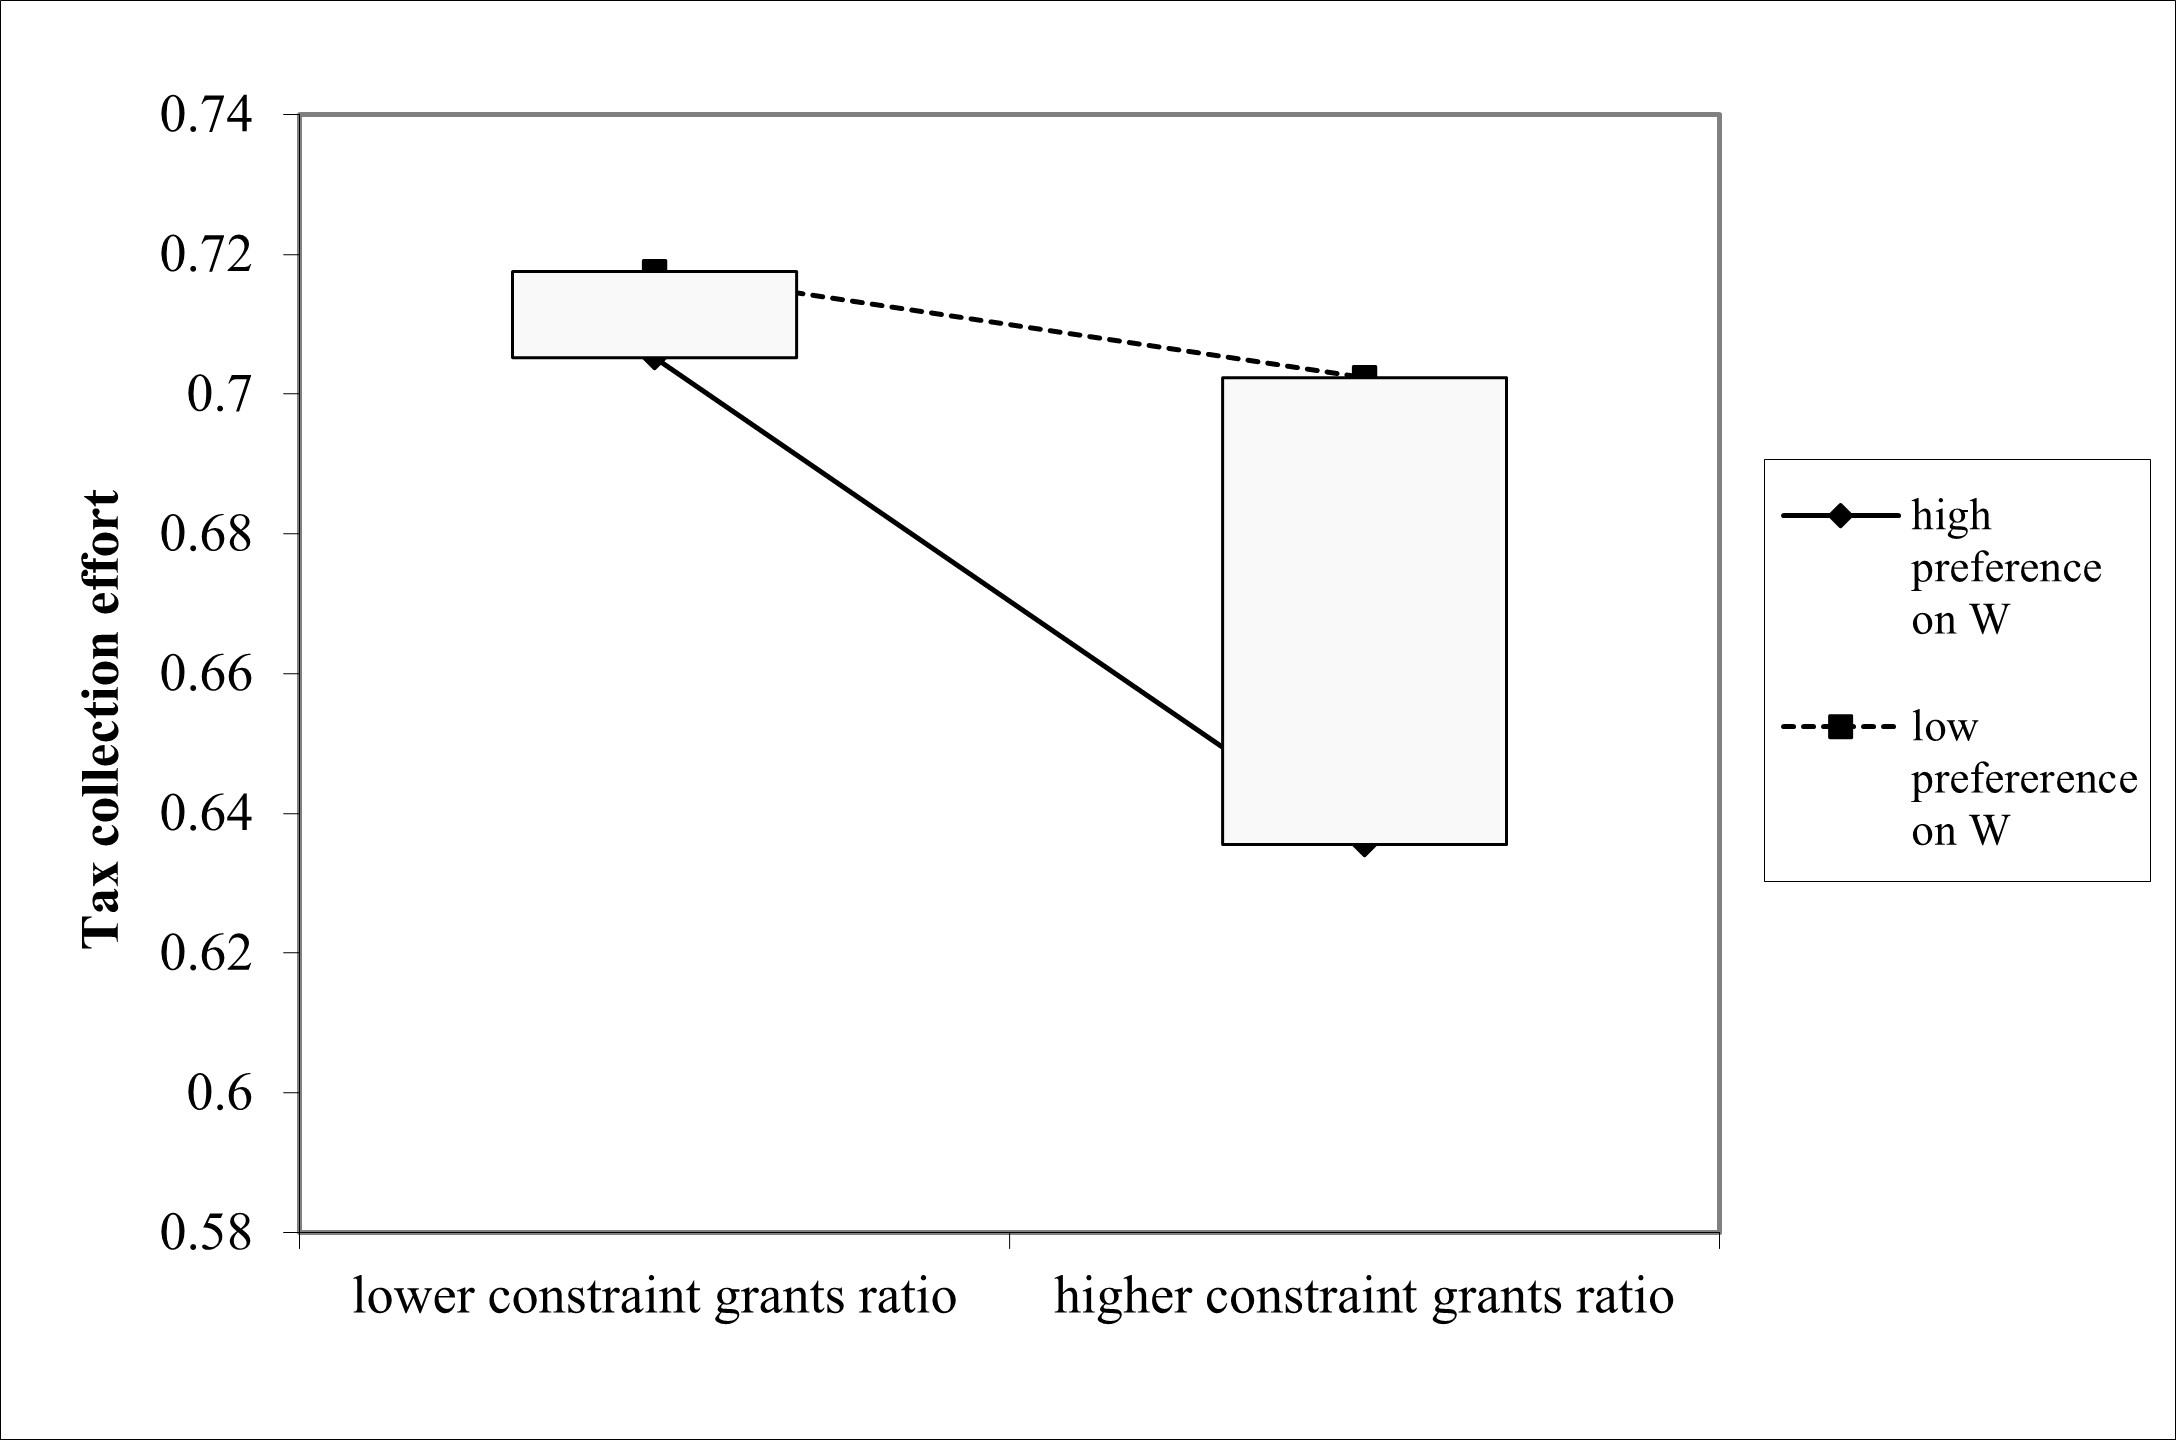
\includegraphics[scale=0.8]{Chapter-5/Figures/inter_cons_W.jpg}
    \caption[Interaction effect between productive categorical transfer ratio and W-preference]{Interaction effect between productive categorical transfer ratio and W-preference
        \texttt{} }
    \label{int_cons_W}
\end{figure}
